\documentclass[12pt,a4paper]{report}

\usepackage[utf8]{inputenc}
\usepackage[OT1]{fontenc}
\usepackage[spanish,es-tabla]{babel}
\usepackage[left=3cm,right=3cm,top=2.5cm,bottom=2.5cm]{geometry}
\usepackage{setspace}
\onehalfspacing
\usepackage{graphicx}
\usepackage{caption}
\captionsetup[figure]{font=normalsize,labelfont=bf,labelsep=colon,justification=centering,singlelinecheck=false}
\captionsetup[table]{labelfont=bf,labelsep=colon,justification=centering,singlelinecheck=false}
\usepackage{tikz}
\usepackage{pgfplots}
\pgfplotsset{compat=1.18}
\usetikzlibrary{arrows.meta,positioning,babel}
\usepackage{booktabs}
\usepackage{longtable}
\usepackage{float}
\usepackage{array}
\usepackage{tabularx}
\newcolumntype{C}{>{\centering\arraybackslash}X}
\usepackage{amsmath,amssymb}
\usepackage{enumitem}
% Viñetas cuadradas pequeñas, con el texto a 2 cm del margen del cuerpo.
\setlist[itemize]{label=\raisebox{0.2ex}{\rule{3.5pt}{3.5pt}},leftmargin=2cm,labelsep=0.25cm,itemsep=0.5\baselineskip,parsep=0pt,topsep=0.5\baselineskip,partopsep=0pt}
\usepackage{microtype}
\usepackage{csquotes}
\DeclareQuoteStyle{spanish}{\textquotedblleft}{\textquotedblright}{\textquoteleft}{\textquoteright}
\usepackage{xurl}
\usepackage{titlesec}
\setlength{\parskip}{0.5\baselineskip plus 2pt minus 1pt}
\setlength{\emergencystretch}{3em}
\widowpenalty=10000
\clubpenalty=10000
\usepackage[backend=bibtex,bibstyle=numeric,citestyle=ieee,sorting=none,giveninits=true,maxbibnames=10,minbibnames=6]{biblatex}
\addbibresource{bibliografia.bib}
\usepackage[colorlinks=true,linkcolor=black,citecolor=black,urlcolor=blue]{hyperref}
\AtBeginBibliography{%
  \hypersetup{urlcolor=blue,citecolor=black,linkcolor=black}%
  \setlength{\bibitemsep}{0.35\baselineskip}%
}
\setcounter{tocdepth}{2}
\titleformat{\chapter}[hang]{\normalfont\Large\bfseries\raggedright}{\thechapter.}{0.6em}{}
\titleformat{\section}{\normalfont\large\bfseries\raggedright}{\thesection.}{0.6em}{}
\titleformat{\subsection}{\normalfont\normalsize\bfseries\raggedright}{\thesubsection.}{0.6em}{}
\titleformat{\subsubsection}{\normalfont\normalsize\bfseries\raggedright}{\thesubsubsection.}{0.6em}{}
\titlespacing*{\chapter}{0pt}{-15pt}{24pt}
\titlespacing*{\section}{0pt}{24pt plus 3pt minus 2pt}{12pt}
\titlespacing*{\subsection}{0pt}{16pt plus 2pt minus 1pt}{10pt}
\titlespacing*{\subsubsection}{0pt}{12pt plus 2pt minus 1pt}{8pt}

\addto\captionsspanish{%
  \renewcommand{\listtablename}{Lista de Tablas}%
  \renewcommand{\listfigurename}{Lista de Figuras}%
}
\makeatletter
\renewcommand{\listoftables}{%
  \chapter*{\listtablename}%
  \addcontentsline{toc}{chapter}{\listtablename}%
  \@starttoc{lot}%
}
\renewcommand{\listoffigures}{%
  \chapter*{\listfigurename}%
  \addcontentsline{toc}{chapter}{\listfigurename}%
  \@starttoc{lof}%
}
\makeatother

\begin{document}
\raggedbottom
\pagenumbering{roman}
\begin{titlepage}
\setlength{\parskip}{0pt}
\centering

\includegraphics[width=0.39\textwidth]{Figuras/00-portada/logo_azul_vert_hipng.png}\par\vspace{0.6cm}
{\Large Universidad de San Andrés\par}\vspace{0.65cm}
{\large Escuela de Ingeniería\par}\vspace{0.65cm}
{\large Ingeniería en Inteligencia Artificial\par}\vspace{1.1cm}
\rule{\textwidth}{0.8pt}\par\vspace{0.5cm}
{\Large Trabajo de Graduación\par}\vspace{0.8cm}
{\LARGE\bfseries Adaptación de modelos de lenguaje a dominios abiertos: aprendizaje por refuerzo guiado por rúbricas extraídas y scaffolding\par}\vspace{0.65cm}
\rule{\textwidth}{0.8pt}\par
\vfill
{\raggedright
\textbf{Autor:} Matías Luciano Antezana\par\vspace{0.4cm}
\textbf{Legajo:} 34581\par\vspace{0.5cm}
\textbf{Mentor:} Dr. Luciano Manuel del Corro\par\vspace{0.3cm}
\textbf{Comentor:} Andrés Arpi\par}
\vfill
Victoria, Buenos Aires\par\vspace{0.5cm}
Noviembre de 2026
\end{titlepage}

\chapter*{Resumen}
\addcontentsline{toc}{chapter}{Resumen}
El aprendizaje por refuerzo con recompensas verificables permite mejorar modelos de lenguaje en tareas con respuestas comprobables, como matemática y programación. Sin embargo, su aplicación a dominios abiertos requiere evaluar respuestas que admiten distintas formulaciones válidas y cuya calidad depende del contexto y de la información incluida. Este trabajo propone una metodología de adaptación que combina ajuste fino supervisado (SFT), rúbricas extraídas de respuestas de referencia y optimización mediante Group Relative Policy Optimization (GRPO). La evaluación integra comprobaciones programáticas y un modelo de lenguaje como juez semántico, mientras las ayudas proporcionadas al modelo se retiran progresivamente durante el entrenamiento.

Una primera evaluación en el dominio clínico utilizó Qwen2.5-7B para estudiar la integración de estos componentes. La comparación en HealthBench entre SFT-90 y SFT-90 + GRPO mostró aumentos de 4,58 puntos porcentuales en seguimiento de instrucciones y de 3,66 en comprensión del contexto, junto con una disminución de 4,11 puntos en calidad de comunicación. Asimismo, el modelo con GRPO cumplió más criterios positivos, pero también activó más criterios negativos. Estos resultados aportaron evidencia inicial sobre los alcances de la metodología y orientaron el refinamiento de las rúbricas y de la recompensa.

A partir de estos hallazgos, la segunda etapa utiliza preguntas y respuestas procedentes de Rubrics as Rewards (RaR) para construir criterios vinculados a las obligaciones de cada consulta y estudiar su puntuación. Se emplea Qwen2.5-3B, partiendo de SFT45k, adaptado mediante QLoRA y actualización de embeddings durante dos épocas sobre 45.000 ejemplos. Los datos de RaR se utilizan por separado para las rúbricas y GRPO. Para contrastar la metodología propuesta con la del paper, el diseño experimental distribuye el conjunto de aprendizaje en un 50\% para SFT y un 50\% para GRPO, con validación y prueba independientes. El contraste se centra en las rúbricas y la recompensa; los modelos de ambas etapas no se comparan directamente.

\bigskip
\noindent\textbf{Palabras clave:} adaptación de dominio, modelos de lenguaje, aprendizaje por refuerzo, rúbricas, GRPO, scaffolding.
\clearpage
%
\chapter*{Abstract}
\addcontentsline{toc}{chapter}{Abstract}
\begin{otherlanguage}{english}
Reinforcement learning with verifiable rewards enables improvements in language models on tasks with checkable answers, such as mathematics and programming. However, applying it to open-ended domains requires evaluating responses that admit different valid formulations and whose quality depends on context and information coverage. This work proposes an adaptation methodology combining supervised fine-tuning (SFT), rubrics extracted from reference answers, and Group Relative Policy Optimization (GRPO). Evaluation integrates programmatic checks and a language model acting as a semantic judge, while hints provided to the model are progressively withdrawn during training.

An initial evaluation in the clinical domain used Qwen2.5-7B to study the integration of these components. A comparison on HealthBench between SFT-90 and SFT-90 + GRPO showed increases of 4.58 percentage points in instruction following and 3.66 points in context awareness, alongside a decrease of 4.11 points in communication quality. Likewise, the GRPO model satisfied more positive criteria but also triggered more negative criteria. These results provided initial evidence of the methodology's capabilities and limitations and guided refinements to rubric construction and reward formulation.

Building on these findings, the second stage uses question--answer pairs from Rubrics as Rewards (RaR) to construct criteria linked to the requirements of each query and investigate their scoring. This stage employs Qwen2.5-3B, starting from SFT45k, adapted through QLoRA and embedding updates over two epochs on 45,000 examples. RaR-derived data are used separately for rubric construction and GRPO. To contrast the proposed methodology with the approach used in the paper, the experimental design allocates 50\% of the learning dataset to SFT and 50\% to GRPO, with independent validation and test sets. The comparison focuses on rubrics and reward formulation; models from the two research stages are not compared directly.

\bigskip
\noindent\textbf{Keywords:} domain adaptation, language models, reinforcement learning, rubrics, GRPO, scaffolding.
\end{otherlanguage}
\clearpage
%
\chapter*{Agradecimientos}
\addcontentsline{toc}{chapter}{Agradecimientos}
Quiero agradecer, en primer lugar, a mi mentor, el Dr. Luciano Manuel del Corro, y a mi comentor, Andrés Arpi, por acompañarme a lo largo de este proyecto, por su disponibilidad y apoyo constantes, por dedicar tiempo a discutir y validar los métodos que fui empleando y por ayudarme a revisar y reformular el trabajo en los momentos de dificultad, especialmente cuando necesitaba definir con mayor claridad la metodología y justificar las decisiones del entrenamiento, así como a Luciano por facilitar los recursos de cómputo que hicieron posible llevar a cabo los experimentos.

También agradezco a Matías Perlin, docente del Taller de Proyecto Final, y a Roberto Bunge, docente y director de la carrera, por sus orientaciones para organizar las distintas etapas de la tesis, desde la elaboración del informe y la planificación de los plazos hasta la preparación de las presentaciones orales, y por sus devoluciones durante este proceso.

A la Universidad de San Andrés y, en especial, a la Escuela de Ingeniería, por la formación que recibí durante estos años y por brindar el espacio para desarrollar este proyecto. A sus docentes, por compartir sus conocimientos y por enseñarme a abordar los problemas con curiosidad y rigor.

A mis amigos y compañeros, por la compañía, el intercambio de ideas y el apoyo durante la carrera, y por ayudarme en los momentos en que me costó formular con claridad la metodología del proyecto, escuchando mis ideas y compartiendo sus observaciones.

Por último, agradezco a todas las personas que, de una forma u otra, contribuyeron a mi formación y a la realización de este trabajo.
\clearpage
%

\tableofcontents
\clearpage
\listoftables
\clearpage
\listoffigures
\clearpage
\begingroup
\titleformat{\chapter}[hang]{\normalfont\Large\bfseries\raggedright}{\thechapter.}{0.6em}{}
\chapter*{Lista de símbolos y abreviaciones}
\addcontentsline{toc}{chapter}{Lista de símbolos y abreviaciones}

\raggedright
\setlength{\parskip}{0pt}
\renewcommand{\arraystretch}{1.25}
\noindent
\begin{tabularx}{\textwidth}{@{}>{\bfseries}p{1.6cm}>{\raggedright\arraybackslash}X@{}}
IA & Inteligencia artificial \\
LLM & Large Language Model (modelo de lenguaje de gran escala) \\
SFT & Supervised Fine-Tuning (ajuste fino supervisado) \\
RL & Reinforcement Learning (aprendizaje por refuerzo) \\
GRPO & Group Relative Policy Optimization (optimización de políticas relativa a grupos) \\
RLVR & Reinforcement Learning with Verifiable Rewards (aprendizaje por refuerzo con recompensas verificables) \\
RLHF & Reinforcement Learning from Human Feedback (aprendizaje por refuerzo a partir de retroalimentación humana) \\
PPO & Proximal Policy Optimization (optimización proximal de políticas) \\
LoRA & Low-Rank Adaptation (adaptación de bajo rango) \\
IC & Intervalo de confianza \\
\end{tabularx}
\endgroup
%

\clearpage
\pagenumbering{arabic}
\chapter{Introducción}
\label{ch:introduccion}
\section{Revolución del aprendizaje por refuerzo}

El aprendizaje por refuerzo permite mejorar las respuestas de un modelo de lenguaje a partir de la evaluación de sus propios intentos. Cuando una solución puede comprobarse, como ocurre en determinados problemas matemáticos o tareas de programación, esa verificación proporciona una señal de recompensa para orientar el aprendizaje. El aprendizaje por refuerzo con recompensas verificables (RLVR) convierte así la capacidad de comprobar resultados en una herramienta de entrenamiento~\cite{shao2024deepseekmath,deepseek2025r1}. Un ejemplo de este avance es DeepSeek-R1-Zero, cuyo entrenamiento mediante Group Relative Policy Optimization (GRPO) con recompensas basadas en reglas elevó el desempeño en problemas matemáticos de AIME 2024 del 15,6\,\% al 71,0\,\% en la métrica pass@1, sin una etapa inicial de ajuste fino supervisado~\cite{deepseek2025r1}.

Sin embargo, trasladar estos avances a dominios abiertos plantea una dificultad: ¿cómo orientar el aprendizaje cuando la calidad de una respuesta no puede comprobarse por completo mediante reglas deterministas? Esta pregunta motiva el presente trabajo, que propone una metodología de adaptación basada en rúbricas extraídas automáticamente de respuestas de referencia y en ayudas que se retiran progresivamente durante el entrenamiento.
%
\section{Adaptación a dominios abiertos mediante rúbricas}

En los dominios abiertos, una misma consulta puede admitir múltiples respuestas válidas, cuyo valor depende del contexto, de la información incluida y de cómo se relacionan los conceptos. A diferencia de las tareas con una solución verificable, no suele existir una regla única que permita determinar si una respuesta es correcta en su conjunto. Aun así, algunos aspectos pueden verificarse, como la presencia de información relevante, el cumplimiento de ciertas restricciones o la inclusión de conceptos esperados, lo que ofrece un punto de partida para el entrenamiento. Para comprobar estos aspectos, es necesario reconocer que una misma idea puede expresarse de distintas maneras y que la presencia de un término no garantiza su uso adecuado en el contexto.

Para abordar esta dificultad, la metodología parte de una adaptación mediante ajuste fino supervisado (SFT) y utiliza respuestas de referencia de una partición reservada para extraer automáticamente las rúbricas, que reúnen los conceptos relevantes para cada consulta. La evaluación combina comprobaciones mediante código con un modelo de lenguaje que actúa como juez semántico, examinando los conceptos no detectados por esas comprobaciones para reconocer formulaciones equivalentes. A partir de esta evaluación se construye la recompensa que orienta el aprendizaje por refuerzo. Durante el entrenamiento, parte de los conceptos se presenta al modelo como ayuda y se retira progresivamente, mientras la rúbrica completa se conserva para evaluar sus respuestas. La figura~\ref{fig:intro-pipeline} resume este procedimiento.

\begin{figure}[H]
\centering
\begingroup
\singlespacing
\shorthandoff{<>}
\definecolor{pipelineink}{HTML}{253F53}
\definecolor{pipelineline}{HTML}{658AA8}
\definecolor{pipelinepaper}{HTML}{F7FAFC}
\definecolor{pipelineblue}{HTML}{C7DCEC}
\definecolor{pipelinepale}{HTML}{DBE7F0}
\definecolor{pipelineshadow}{HTML}{D6E0E8}
% Tarjeta vectorial con cabecera, cuerpo y sombra discreta.
\newcommand{\pipelinecard}[8]{%
 \fill[pipelineshadow,rounded corners=7pt]
 ({#2-#4/2-.055},{#3-#5/2-.075}) rectangle
 ({#2+#4/2-.055},{#3+#5/2-.075});
 \node[draw=pipelineline,fill=pipelinepaper,rounded corners=7pt,
   line width=.85pt,minimum width=#4cm,minimum height=#5cm,inner sep=0pt]
   (#1) at (#2,#3) {};
 \draw[draw=pipelineline,fill=#8,rounded corners=5pt,line width=.7pt]
 ({#2-#4/2+.13},{#3+#5/2-.55}) rectangle
 ({#2+#4/2-.13},{#3+#5/2-.13});
 \node[font=\sffamily\footnotesize\bfseries,text=pipelineink,align=center,inner sep=0pt]
 at (#2,{#3+#5/2-.34}) {#6};
 \node[font=\sffamily\small,text=pipelineink,align=center,inner sep=0pt]
 at (#2,{#3-.27}) {#7};
}
\resizebox{\textwidth}{!}{%
\begin{tikzpicture}[>=Stealth,
 flow/.style={->,draw=pipelineline,line width=1pt,rounded corners=4pt,line join=round},
 label/.style={font=\sffamily\footnotesize,fill=white,inner sep=3pt,text=pipelineink}]
\pipelinecard{data}{0}{0}{2.3}{1.95}{Consultas y}{respuestas\\del dominio}{pipelinepale}
\pipelinecard{sft}{2.9}{1.8}{2.1}{1.45}{Datos}{para SFT}{pipelineblue}
\pipelinecard{reserve}{2.9}{-1.8}{2.1}{1.95}{Datos}{reservados\\para GRPO}{pipelineblue}
\pipelinecard{model}{5.9}{1.8}{3.05}{1.45}{Entrenamiento}{con SFT}{pipelineblue}
\pipelinecard{extractor}{5.9}{-1.8}{2.4}{1.95}{LLM}{Extracción de\\criterios}{pipelinepale}
\pipelinecard{rubric}{8.9}{-1.8}{2.25}{1.45}{Rúbricas}{extraídas}{pipelinepale}
\fill[pipelineshadow,rounded corners=7pt] (10.62,-2.6) rectangle (13.07,-1.15);
\node[draw=pipelineline,fill=pipelinepaper,rounded corners=7pt,line width=.85pt,
 minimum width=2.45cm,minimum height=1.45cm,inner sep=0pt] (scaffold) at (11.9,-1.8) {};
\draw[draw=pipelineline,fill=pipelineblue,rounded corners=5pt,line width=.7pt]
 (10.805,-2.01) rectangle (12.995,-1.59);
\node[font=\sffamily\footnotesize\bfseries,text=pipelineink,inner sep=0pt]
 at (11.9,-1.8) {Scaffolding};
\pipelinecard{grpo}{15.1}{0}{3.05}{1.95}{Entrenamiento}{con GRPO\\con rúbricas}{pipelineblue}
\pipelinecard{final}{18.3}{0}{2.1}{1.45}{Modelo}{Final}{pipelineblue}
\draw[flow] (data.east) -- (1.5,0) |- (sft.west);
\draw[flow] (1.5,0) |- (reserve.west);
\draw[flow] (sft.east) -- (model.west);
\draw[flow] (reserve.east) -- (extractor.west);
\draw[flow] (extractor.east) -- (rubric.west);
\draw[flow] (reserve.north) -- (2.9,-.25) --
 node[label,above]{Consultas} (11.9,-.25) -- (scaffold.north);
\draw[flow] (rubric.east) -- (scaffold.west);
\draw[flow] (model.east) -| (grpo.north);
\draw[flow] (scaffold.east) -- (13.35,-1.8) |- (grpo.west);
\draw[flow] (rubric.south) -- (8.9,-3.2) --
 node[label,above]{Rúbrica completa} (15.1,-3.2) -- (grpo.south);
\draw[flow] (grpo.east) -- (final.west);
\end{tikzpicture}%
}
\endgroup

\caption{Metodología de adaptación mediante SFT y GRPO, con rúbricas extraídas de respuestas de referencia, evaluación híbrida y retirada progresiva de ayudas.}
\label{fig:intro-pipeline}
\end{figure}

Los trabajos previos abordan distintos componentes de este procedimiento. Rubicon estudia las rúbricas como señal de recompensa~\cite{huang2025rubicon}, mientras que ARES automatiza la construcción de preguntas, respuestas y criterios a partir de documentos~\cite{li2026ares} y RuscaRL incorpora ayudas basadas en rúbricas que se retiran progresivamente~\cite{zhou2026ruscarl}. Frente a estos antecedentes, el presente trabajo aprovecha pares de consulta y respuesta existentes para realizar la adaptación supervisada y extraer criterios de una partición reservada, independiente del benchmark externo. Su aporte se concentra en integrar la evaluación híbrida y la retirada progresiva de ayudas en ese procedimiento de adaptación de dominio.

El dominio clínico ofrece un caso de estudio relevante para esta metodología, porque sus consultas requieren respuestas abiertas que combinan conocimientos especializados con información propia de cada situación. Evaluarlas exige considerar tanto los conceptos incluidos como las posibles omisiones y la adecuación de las recomendaciones al contexto~\cite{arora2025healthbench}. Por ello, las consultas clínicas permiten estudiar si la recompensa favorece respuestas que recuperan información relevante y la utilizan adecuadamente en el contexto del paciente.

Para estudiar los efectos del entrenamiento, la evaluación compara el modelo adaptado mediante SFT con su posterior optimización mediante aprendizaje por refuerzo guiado por rúbricas. Para ello, se utiliza HealthBench como evaluación externa, con rúbricas independientes de las empleadas durante el entrenamiento~\cite{arora2025healthbench}. El análisis examina los cambios en distintas dimensiones de las respuestas y se complementa con ejemplos que permiten identificar mejoras, regresiones y limitaciones de la propuesta.


La investigación se desarrolla en dos etapas. En la primera, los experimentos con Qwen2.5-7B permitieron evaluar la integración inicial de SFT, rúbricas y GRPO e identificar mejoras en algunas dimensiones junto con regresiones y limitaciones del evaluador. A partir de esos aprendizajes, la segunda etapa utiliza preguntas y respuestas procedentes de Rubrics as Rewards (RaR) para construir nuevas rúbricas y estudiar distintas formas de puntuarlas~\cite{gunjal2025rar}. Esta etapa trabaja con Qwen2.5-3B y otro diseño experimental; su relación con la evaluación inicial es metodológica, como se precisa en la sección~\ref{sec:resultados-modelos}.
%
\section{Objetivos y aportes: Metodología de adaptación de dominio mediante rúbricas y scaffolding progresivo}

El objetivo de este trabajo es desarrollar y evaluar una metodología de adaptación de modelos de lenguaje a dominios abiertos mediante aprendizaje por refuerzo guiado por rúbricas extraídas automáticamente de respuestas de referencia.

A partir de este objetivo general, se plantean los siguientes objetivos específicos:

\begin{itemize}
\item \textbf{Establecer una adaptación inicial al dominio:} ajustar un modelo de lenguaje mediante entrenamiento supervisado con consultas y respuestas del dominio, reservando una partición independiente para construir las rúbricas del entrenamiento posterior.
\item \textbf{Construir una señal de recompensa basada en rúbricas:} extraer conceptos relevantes de las respuestas de referencia de la partición reservada y organizarlos en criterios específicos por consulta, combinando comprobaciones mediante código con evaluación semántica.
\item \textbf{Integrar las rúbricas y el scaffolding en la optimización con GRPO:} implementar un entrenamiento por refuerzo que retire progresivamente las ayudas proporcionadas al modelo, manteniendo la rúbrica completa para evaluar sus respuestas y una recompensa que favorezca la recuperación de información no presentada como ayuda.
\item \textbf{Evaluar los alcances y las limitaciones de la metodología:} examinar inicialmente el modelo adaptado mediante SFT y su posterior optimización mediante GRPO utilizando HealthBench como evaluación externa, analizando los cambios por dimensiones y ejemplos de respuestas que permitan identificar mejoras y regresiones.
\item \textbf{Refinar las rúbricas y contrastar su uso como recompensa:} estudiar una nueva construcción de criterios a partir de preguntas y respuestas procedentes de RaR y variantes de puntuación, documentando las diferencias de modelo, datos y evaluación que condicionan el contraste con ese antecedente.
\end{itemize}

Se conservan las configuraciones y los registros de entrenamiento y evaluación para revisar las decisiones experimentales.
%
\section{Organización del documento}
El capítulo~\ref{ch:marco-teorico} reúne los fundamentos de adaptación de dominio, SFT y aprendizaje por refuerzo, con especial atención a PPO y GRPO. También presenta las rúbricas, los modelos de lenguaje como jueces y la evaluación en HealthBench.

El capítulo~\ref{ch:metodo-propuesto} desarrolla la construcción de rúbricas, la evaluación de criterios y la retirada progresiva de ayudas, junto con las arquitecturas, la configuración de entrenamiento y las métricas utilizadas. A continuación, el capítulo~\ref{ch:evolucion-entrenamiento} describe los datos y analiza las curvas disponibles de aprendizaje en las dos etapas de investigación.

El capítulo~\ref{ch:resultados-adaptacion} presenta la evaluación de los modelos en HealthBench, el alcance del contraste con RaR y el análisis de respuestas concretas. Finalmente, el capítulo~\ref{ch:contribuciones} reúne las contribuciones del trabajo y las líneas de evaluación pendientes.
%

\chapter{Marco teórico}
\label{ch:marco-teorico}
Este capítulo reúne los fundamentos necesarios para comprender la adaptación de modelos de lenguaje mediante entrenamiento supervisado y aprendizaje por refuerzo. El recorrido comienza con la adaptación de dominio y el post training, desarrolla las señales de aprendizaje y los algoritmos PPO y GRPO, y presenta después las rúbricas, los modelos jueces y la evaluación externa. Las configuraciones de los experimentos se describen junto con su aplicación y sus resultados.

\section{Adaptación de dominio y post training}
\label{sec:marco-post-training}
Durante el preentrenamiento, un modelo de lenguaje desarrolla capacidades generales a partir de grandes corpus, mientras que la adaptación de dominio busca orientar esas capacidades hacia el vocabulario, los conocimientos y las tareas de un ámbito específico. En este contexto, el proceso de post training puede combinar demostraciones supervisadas con la evaluación de respuestas generadas por el propio modelo, de modo que cada etapa aporta una señal de aprendizaje diferente~\cite{gururangan2020dontstop,ouyang2022instructgpt}.

Dentro de las estrategias de adaptación, el preentrenamiento adaptativo al dominio (DAPT) continúa el aprendizaje sobre textos especializados, mientras que la adaptación al corpus de una tarea (TAPT) utiliza textos asociados a esa tarea~\cite{gururangan2020dontstop}. Por su parte, el SFT utiliza demostraciones explícitas de cómo responder, de manera que incorporar documentos del área y entrenar con pares de consulta y respuesta no constituye el mismo procedimiento. En consecuencia, su alcance depende de la calidad y la cobertura de las referencias, cuyos errores u omisiones también pueden aprenderse.

La elección de la señal depende también de la tarea. En problemas con resultados verificables puede utilizarse una regla que compruebe la solución, mientras que en dominios abiertos algunos aspectos admiten comprobaciones automáticas y otros requieren interpretar el contenido y el contexto~\cite{deepseek2025r1,arora2025healthbench}. Esta diferencia motiva estudiar cómo construir recompensas a partir de criterios explícitos, después de establecer los fundamentos del ajuste supervisado y del aprendizaje por refuerzo.
%
\section{Ajuste fino supervisado}
\label{sec:marco-sft}
\subsection{Objetivo y funcionamiento del ajuste fino supervisado}
\label{sec:sft-objetivo}
El ajuste fino supervisado, conocido como Supervised Fine-Tuning (SFT), utiliza demostraciones para orientar un modelo hacia una tarea, un formato de interacción o un dominio. Su punto de partida son parámetros obtenidos durante el preentrenamiento, que se ajustan con un conjunto de ejemplos de entrada y respuesta~\cite{ouyang2022instructgpt}, representado como
\begin{equation}
\mathcal{D}_{\mathrm{SFT}}=\{(x_i,y_i)\}_{i=1}^{N},
\label{eq:datos-sft}
\end{equation}
donde $x_i$ reúne la instrucción, la consulta y el contexto disponible, $y_i$ es la respuesta de referencia y $N$ indica la cantidad de ejemplos. El entrenamiento busca aumentar la probabilidad de esas respuestas condicionadas a sus entradas, por lo que las demostraciones determinan qué contenido y qué formas de respuesta se favorecen.


%
\subsection{Preparación de ejemplos y predicción autorregresiva}
\label{sec:sft-ejemplos}
Antes de entrenar, cada ejemplo se transforma en una secuencia de tokens mediante el tokenizador del modelo. En un formato conversacional, una plantilla organiza las instrucciones y los mensajes e incorpora delimitadores de roles, por lo que deben respetarse las convenciones del modelo de partida. Si $T_i$ es la longitud de la respuesta $i$, su probabilidad se descompone en predicciones del token siguiente,
\begin{equation}
p_\theta(y_i\mid x_i)=\prod_{t=1}^{T_i}
p_\theta(y_{i,t}\mid x_i,y_{i,<t}),
\label{eq:sft-autorregresivo}
\end{equation}
donde $\theta$ representa los parámetros del modelo y $y_{i,<t}$ contiene los tokens anteriores de la respuesta. Esta distribución es la que, en la sección~\ref{sec:marco-rl}, se interpretará como política y se denotará por $\pi_\theta$.

Durante el entrenamiento se aplica teacher forcing, una técnica que utiliza los tokens anteriores de la respuesta de referencia como contexto para predecir el siguiente token. En cada posición, el modelo recibe la consulta y la parte de la referencia que precede al token esperado, y la pérdida compara la distribución que produce con ese token correcto. Así, aunque asigne mayor probabilidad a un token incorrecto, las predicciones siguientes siguen utilizando el historial de la referencia. En cambio, durante la generación, el contexto se amplía con los tokens que el propio modelo va produciendo, de modo que un error puede influir en las predicciones posteriores.

Como la referencia completa está disponible durante el entrenamiento, un Transformer causal puede calcular las predicciones de distintas posiciones en paralelo, utilizando una máscara de atención que impide acceder a los tokens futuros~\cite{vaswani2017attention}. La figura~\ref{fig:sft-secuencia} muestra cómo se organizan el contexto, la respuesta y el relleno, distinguiendo qué información utiliza el modelo de qué posiciones se supervisan.

\begin{figure}[htbp]
\centering
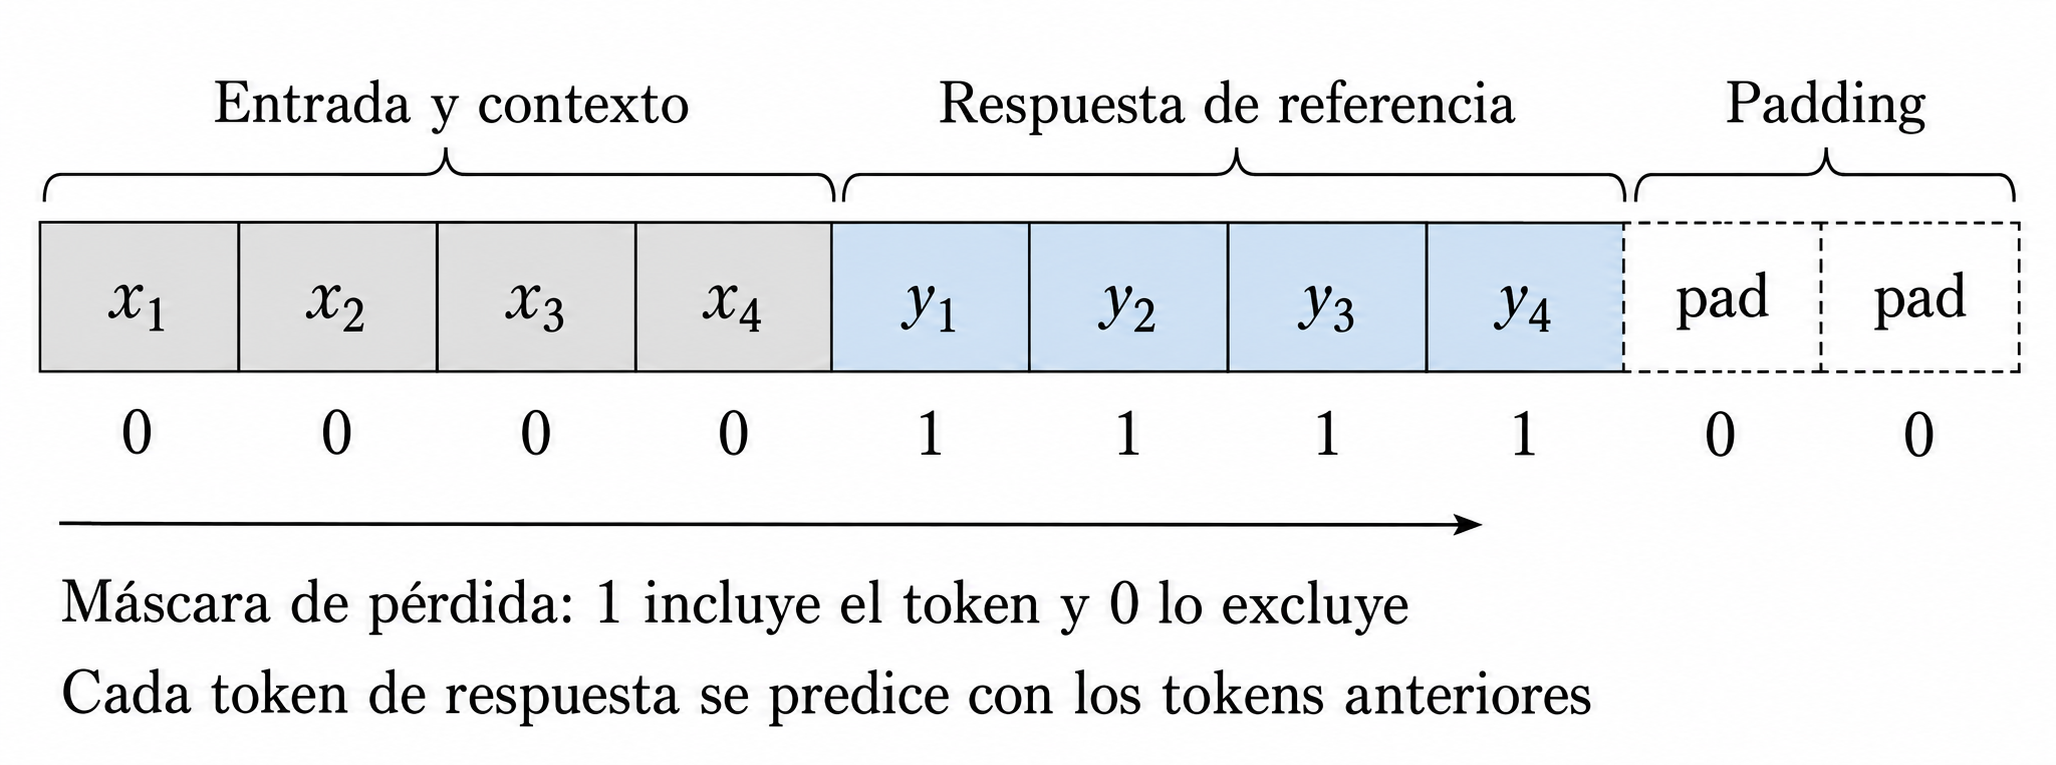
\includegraphics[width=0.95\textwidth]{Figuras/02-marco-teorico/02-ajuste-supervisado/sft-secuencia-tokens.png}
\caption{Secuencia de tokens con pérdida calculada únicamente sobre la respuesta.}
\label{fig:sft-secuencia}
\end{figure}

La preparación también requiere separar entrenamiento y validación, comprobar duplicados y evitar que una misma consulta o una variante cercana aparezca en ambos conjuntos. Asimismo, el límite de secuencia comprende la entrada y la respuesta, por lo que el truncamiento puede eliminar contexto o contenido supervisado y debe registrarse como parte del procedimiento. Este límite difiere de la cantidad máxima de tokens nuevos que se permite generar durante la inferencia, mientras que el padding permite reunir secuencias de longitudes distintas en un batch y se excluye de la pérdida para que el relleno no se aprenda como respuesta.

%
\subsection{Función de pérdida y actualización de parámetros}
\label{sec:sft-actualizacion}
Para el caso en que se supervisan únicamente los tokens de respuesta, la función de pérdida puede escribirse como el logaritmo de verosimilitud negativo promediado sobre esos tokens,
\begin{equation}
\mathcal{L}_{\mathrm{SFT}}(\theta)=
-\frac{1}{\sum_{i=1}^{N}T_i}
\sum_{i=1}^{N}\sum_{t=1}^{T_i}
\log p_\theta(y_{i,t}\mid x_i,y_{i,<t}).
\label{eq:sft}
\end{equation}
Esta expresión corresponde a una entropía cruzada con el token de referencia como etiqueta y penaliza que el modelo le asigne una probabilidad baja. En esta formulación, el promedio por tokens hace que una respuesta más larga aporte más términos al conjunto, por lo que no equivale a promediar primero la pérdida de cada respuesta y luego dar el mismo peso a todos los ejemplos. La maximización de probabilidades condicionales constituye el objetivo supervisado, independientemente de qué parámetros se permitan modificar~\cite{hu2022lora}.

Para expresar explícitamente la selección de posiciones, sea $z_i$ la secuencia completa del ejemplo y $m_{i,t}\in\{0,1\}$ una máscara que indica si el token en la posición $t$ contribuye a la pérdida. Entonces,
\begin{equation}
\mathcal{L}_{\mathrm{SFT}}(\theta)=
-\frac{\sum_{i,t}m_{i,t}\log p_\theta(z_{i,t}\mid z_{i,<t})}
{\sum_{i,t}m_{i,t}},
\label{eq:sft-mascara}
\end{equation}
siempre que exista al menos un token supervisado. En el ejemplo de la figura \ref{fig:sft-secuencia}, la máscara vale uno en la respuesta y cero en el contexto y el padding. Esta máscara de pérdida cumple una función distinta de la máscara causal de atención, ya que un token excluido como objetivo puede seguir proporcionando contexto a las predicciones siguientes.

El entrenamiento procesa un batch, calcula las probabilidades y la pérdida, obtiene sus gradientes por retropropagación y aplica una actualización sobre el subconjunto entrenable $\theta_{\mathrm{train}}$. Una representación básica mediante descenso de gradiente es
\begin{equation}
\theta_{\mathrm{train}}\leftarrow\theta_{\mathrm{train}}
-\eta\,\nabla_{\theta_{\mathrm{train}}}\mathcal{L}_{\mathrm{SFT}},
\label{eq:sft-actualizacion}
\end{equation}
donde $\eta$ es la tasa de aprendizaje. Esta expresión explica la dirección de la actualización, aunque optimizadores como AdamW utilizan además estimaciones de momentos del gradiente y decaimiento de pesos separado de la actualización adaptativa, por lo que su operación no se reduce a ese paso básico~\cite{loshchilov2019adamw}.

El microbatch determina cuántos ejemplos se procesan simultáneamente, mientras que la acumulación de gradientes combina varias operaciones antes de actualizar los parámetros y permite aumentar el batch efectivo bajo restricciones de memoria. Por otra parte, una época corresponde a un recorrido por el conjunto de entrenamiento y la tasa de aprendizaje controla la escala de los cambios, por lo que estas decisiones deben interpretarse junto con la pérdida de validación, cuyo descenso indica un mejor ajuste a las referencias de ese conjunto.

%
\subsection{Entrenamiento de parámetros mediante LoRA}
\label{sec:sft-parametros}
El ajuste completo requiere calcular y almacenar gradientes y estados del optimizador para todos los parámetros del modelo, lo que aumenta el uso de memoria y el costo del entrenamiento. El ajuste parcial reduce esa carga al actualizar solo un subconjunto, aunque la adaptación queda condicionada por las capas o los módulos seleccionados. Frente a estas restricciones, LoRA incorpora matrices entrenables de rango reducido en las proyecciones elegidas y mantiene congelados sus pesos originales~\cite{hu2022lora}.

Como muestra la figura~\ref{fig:sft-parametros}, una misma entrada recorre dos ramas: la transformación original y la actualización de LoRA. Sus salidas se suman, de modo que el modelo puede modificar su respuesta mediante los parámetros añadidos sin actualizar la matriz base.

\begin{figure}[htbp]
\centering
\input{Figuras/02-marco-teorico/02-ajuste-supervisado/sft-lora-parametros}
\caption{LoRA: pesos base congelados y matrices $A$ y $B$ entrenables.}
\label{fig:sft-parametros}
\end{figure}

Para una matriz $W_0\in\mathbb{R}^{d_{\mathrm{out}}\times d_{\mathrm{in}}}$, la transformación utiliza los pesos efectivos
\begin{equation}
W_{\mathrm{eff}}=W_0+\frac{\alpha}{r}BA,
\qquad A\in\mathbb{R}^{r\times d_{\mathrm{in}}},
\qquad B\in\mathbb{R}^{d_{\mathrm{out}}\times r},
\label{eq:sft-lora}
\end{equation}
donde $r$ determina el rango de la actualización y $\alpha/r$ controla su escala. La matriz $A$ proyecta la entrada a una dimensión reducida y $B$ la lleva a la dimensión de salida, mientras $W_0$ permanece fija.

Durante el SFT, la pérdida se calcula sobre las predicciones obtenidas con esta transformación. A continuación, la retropropagación calcula los gradientes de $A$ y $B$, y el optimizador actualiza esas matrices para reducir la pérdida. Los pesos de $W_0$ siguen interviniendo en el cálculo de la salida, pero no reciben actualizaciones. Este procedimiento se aplica a cada proyección seleccionada para incorporar LoRA.

Para esa matriz, la cantidad de parámetros entrenables añadidos es
\begin{equation}
P_{\mathrm{LoRA}}=r(d_{\mathrm{in}}+d_{\mathrm{out}}),
\qquad P_{W_0}=d_{\mathrm{in}}d_{\mathrm{out}},
\label{eq:sft-lora-parametros}
\end{equation}
por lo que un rango pequeño reduce el número de parámetros entrenables y los recursos necesarios para calcular y almacenar sus gradientes y estados del optimizador, disminuyendo así el costo del entrenamiento. La selección de proyecciones, el rango y la escala definen la configuración de los adaptadores.
%
%
\section{Aprendizaje por refuerzo y recompensas verificables}
\label{sec:marco-rl}
En el aprendizaje por refuerzo, la señal procede de evaluar las respuestas que genera el modelo. Para comprender su relación con el SFT, primero se describe la generación de texto como una secuencia de decisiones y después se examinan las fuentes de recompensa.

\subsection{Fundamentos del aprendizaje por refuerzo aplicado al lenguaje}
\label{sec:rl-lenguaje}
El aprendizaje por refuerzo estudia cómo un agente modifica su comportamiento a partir de las consecuencias de sus acciones al interactuar con un entorno, buscando maximizar la recompensa acumulada esperada~\cite{sutton2018reinforcement}. Para elegir una acción, el agente utiliza una política que relaciona el estado disponible con las acciones posibles, mientras que el entorno determina la transición al estado siguiente y las señales de recompensa. De este modo, el aprendizaje depende tanto de las decisiones tomadas como de la evaluación de sus consecuencias, que puede recibirse inmediatamente o después de varias acciones.

En la generación de texto, el modelo de lenguaje actúa como agente y su distribución de probabilidades constituye la política, representada por $\pi_\theta$, donde $\theta$ reúne los parámetros entrenables. Si $x$ es la consulta y $y_{<t}$ contiene los tokens ya generados, el estado en el paso $t$ puede escribirse como $s_t=(x,y_{<t})$, mientras que la acción consiste en seleccionar el token siguiente $y_t$. Por lo tanto, cada elección amplía el contexto disponible para la próxima, y la sucesión de acciones forma una trayectoria que termina cuando se genera el token de fin o se alcanza el límite de longitud. En este caso, el entorno comprende el procedimiento que actualiza el contexto y el mecanismo que evalúa la respuesta, sin que sea necesario interactuar con un paciente real para entrenar sobre consultas almacenadas~\cite{ouyang2022instructgpt}.

Cuando se asigna una recompensa al finalizar la respuesta, un objetivo simplificado consiste en aumentar su valor esperado sobre las consultas de entrenamiento,
\begin{equation}
J(\theta)=\mathbb{E}_{x\sim\mathcal{D},\,y\sim\pi_\theta(\cdot\mid x)}[R(x,y)],
\label{eq:objetivo-rl}
\end{equation}
donde $\mathcal{D}$ representa la distribución de consultas y $R(x,y)$ evalúa la respuesta generada. Esta expresión no incluye todavía las restricciones de estabilidad del algoritmo y tampoco exige una respuesta de referencia única, aunque una referencia puede intervenir en la evaluación. Además de recompensas finales, es posible introducir señales sobre pasos intermedios, lo que permite distinguir la evaluación del resultado de la evaluación del proceso seguido para obtenerlo~\cite{lightman2023verify}.

%
\subsection{Diferencias entre aprendizaje supervisado y aprendizaje por refuerzo}
\label{sec:sft-rl}
La diferencia entre ambos procedimientos se encuentra en la señal que orienta la actualización. En el ajuste fino supervisado, desarrollado en el sección~\ref{sec:marco-sft}, la respuesta de referencia determina los tokens que intervienen en la pérdida de la ecuación \ref{eq:sft}, mientras que en el entrenamiento por refuerzo se evalúan respuestas producidas por la propia política. Esa evaluación proporciona una señal de calidad, pero no necesariamente indica qué token debería haberse generado en cada posición, por lo que el algoritmo debe relacionarla con las probabilidades de las acciones tomadas~\cite{ouyang2022instructgpt}. La figura \ref{fig:sft-rl} permite comparar el origen de las respuestas y el cálculo utilizado para actualizar el modelo.

\begin{figure}[htbp]
\centering
\input{Figuras/02-marco-teorico/04-ppo-grpo/rl-comparacion-sft}
\caption{Comparación entre el ajuste fino supervisado y el aprendizaje por refuerzo.}
\label{fig:sft-rl}
\end{figure}

Ambos procedimientos pueden combinarse cuando el SFT proporciona un comportamiento inicial adecuado y el refuerzo busca ajustar propiedades que la reproducción de demostraciones no controla de manera explícita. Sin embargo, esta secuencia es una decisión de diseño y no una condición general del aprendizaje por refuerzo, como muestra el entrenamiento de DeepSeek-R1-Zero directamente sobre un modelo base~\cite{deepseek2025r1}. La comparación entre SFT y RL debe considerar, por tanto, el punto de partida, los datos y la recompensa utilizados.

%
\subsection{Construcción de la señal de recompensa}
\label{sec:senal-recompensa}
La recompensa expresa qué comportamientos se busca favorecer y cuáles se intenta reducir, por lo que su construcción determina la dirección del entrenamiento. Una posibilidad es obtener evaluaciones humanas sobre respuestas generadas o comparaciones entre pares de respuestas, que permiten aprender un modelo de recompensa capaz de predecir preferencias~\cite{christiano2017preferences,ouyang2022instructgpt}. También puede utilizarse retroalimentación de otros modelos para construir esas preferencias o valorar las respuestas, como ocurre en los procedimientos de aprendizaje con feedback de inteligencia artificial~\cite{bai2022constitutional}. Estas fuentes no son equivalentes, ya que dependen de distintos evaluadores y pueden reproducir sus sesgos.

Cuando existe una condición comprobable, la recompensa puede obtenerse mediante un verificador programático que compare un resultado, ejecute pruebas sobre código o compruebe una restricción de formato~\cite{deepseek2025r1}. Este uso de condiciones comprobables corresponde al aprendizaje por refuerzo con recompensas verificables (RLVR). Una comprobación binaria asigna dos resultados posibles, mientras que una señal graduada permite distinguir niveles de desempeño. Asimismo, la evaluación puede referirse al resultado final o a pasos del razonamiento, una distinción que afecta a la información que recibe el entrenamiento~\cite{lightman2023verify}.

PPO y GRPO utilizan habitualmente una recompensa escalar para calcular la actualización, por lo que el procedimiento de evaluación debe producir un valor que permita comparar las respuestas. Además, el evaluador no necesita ser diferenciable, ya que en los métodos de gradiente de política la señal evaluativa se combina con las probabilidades de las acciones generadas por el modelo~\cite{sutton2018reinforcement}. Por ejemplo, para una recompensa final y una consulta fija, la identidad
\begin{equation}
\nabla_\theta\mathbb{E}_{y\sim\pi_\theta}[R(x,y)]
=\mathbb{E}_{y\sim\pi_\theta}
[R(x,y)\nabla_\theta\log\pi_\theta(y\mid x)]
\label{eq:gradiente-politica}
\end{equation}
muestra que, cuando $R$ se trata como una evaluación fija sin dependencia directa de $\theta$, el gradiente se calcula sobre la política y no atraviesa el juez. Esta relación fundamenta el uso de verificadores y evaluadores externos, aunque los algoritmos prácticos añaden estimadores de ventaja y mecanismos de estabilidad.

%
%
\section{Optimización mediante PPO y GRPO}
\label{sec:marco-optimizacion}
La recompensa orienta la actualización de la política al favorecer las respuestas mejor evaluadas, mientras que PPO y GRPO incorporan mecanismos para controlar esos cambios.

\subsection{Ciclo de optimización y mecanismos de estabilidad}
\label{sec:ciclo-optimizacion}
El ciclo de entrenamiento comienza al seleccionar consultas y generar respuestas mediante una política de muestreo, a partir de las cuales se calculan recompensas y ventajas para actualizar los parámetros. La ventaja indica qué tan favorable resulta una acción o respuesta respecto de una referencia de comparación, lo que permite distinguir una recompensa alta en términos absolutos de una respuesta mejor que las alternativas consideradas. Después de la actualización, se vuelve a generar con la política modificada y se repite el procedimiento, como se representa en la figura \ref{fig:ciclo-rl}~\cite{schulman2017ppo,shao2024deepseekmath}.

\begin{figure}[htbp]
\centering
\input{Figuras/02-marco-teorico/04-ppo-grpo/rl-ciclo-optimizacion}
\caption{Ciclo de generación, evaluación y actualización de la política.}
\label{fig:ciclo-rl}
\end{figure}

Para interpretar este ciclo conviene distinguir la política actual $\pi_\theta$, cuyos parámetros se optimizan, de la política de recolección $\pi_{\mathrm{old}}$, utilizada para generar el conjunto de respuestas de una iteración. Mientras se realizan actualizaciones sobre ese conjunto, ambas pueden diferir, por lo que el algoritmo compara las probabilidades de los tokens bajo las dos políticas. Por otra parte, la política de referencia $\pi_{\mathrm{ref}}$ puede mantenerse fija para regularizar la distancia respecto de un comportamiento inicial, y no debe confundirse con la política que produjo las respuestas de la iteración~\cite{shao2024deepseekmath}.

El muestreo permite obtener distintas respuestas para una misma consulta y, por ello, influye en las alternativas que el entrenamiento puede explorar. Sin embargo, aumentar la diversidad no garantiza que las respuestas sean útiles, mientras que una generación completamente determinista puede reducir la variación necesaria para comparar alternativas. Para controlar la actualización, algunos métodos utilizan clipping sobre la razón de probabilidades y una penalización por divergencia de Kullback y Leibler (KL). El primero limita el incentivo del objetivo a ciertos cambios respecto de la política de recolección, mientras que la segunda penaliza la distancia respecto de una política de referencia, por lo que cumplen funciones distintas y ninguno garantiza por sí solo la estabilidad del entrenamiento~\cite{schulman2017ppo,ouyang2022instructgpt}.

Para un estado fijo $s$, la divergencia KL entre la política actual y la de referencia se define como
\begin{equation}
D_{\mathrm{KL}}\!\left(\pi_\theta(\cdot\mid s)\,\|\,\pi_{\mathrm{ref}}(\cdot\mid s)\right)
=\sum_{a\in\mathcal{V}}\pi_\theta(a\mid s)
\log\frac{\pi_\theta(a\mid s)}{\pi_{\mathrm{ref}}(a\mid s)},
\label{eq:kl}
\end{equation}
donde $\mathcal{V}$ es el vocabulario de tokens y se supone que la política de referencia asigna probabilidad positiva a las acciones consideradas. Esta divergencia compara distribuciones completas y vale cero cuando coinciden, mientras que un coeficiente $\beta$ controla su contribución al objetivo. En implementaciones de entrenamiento puede estimarse mediante los tokens muestreados, por lo que también debe documentarse el estimador utilizado, además del valor de $\beta$~\cite{shao2024deepseekmath}.

%
\subsection{PPO como antecedente de la optimización de modelos de lenguaje}
\label{sec:ppo}
Proximal Policy Optimization (PPO) pertenece a los métodos de optimización de políticas y, en su formulación habitual de actor y crítico, combina una política que selecciona acciones con una función de valor que estima el retorno esperado desde un estado. Esta estimación ayuda a calcular las ventajas utilizadas para actualizar la política, mientras que el crítico se entrena a partir de los retornos observados. Para evitar que la reutilización de las muestras incentive cambios excesivos, una variante de PPO utiliza el objetivo con clipping~\cite{schulman2017ppo},
\begin{equation}
L^{\mathrm{clip}}(\theta)=\mathbb{E}_{t}\!\left[
\min\left(\rho_t(\theta)\widehat{A}_t,
\operatorname{clip}(\rho_t(\theta),1-\epsilon_c,1+\epsilon_c)\widehat{A}_t\right)
\right],
\label{eq:ppo}
\end{equation}
donde $\rho_t(\theta)=\pi_\theta(a_t\mid s_t)/\pi_{\mathrm{old}}(a_t\mid s_t)$ compara la probabilidad de la acción observada, $\widehat{A}_t$ es su ventaja estimada y $\epsilon_c$ determina el intervalo de recorte. De este modo, cuando el cambio de probabilidad ya favorece suficientemente una acción con ventaja positiva, el objetivo deja de premiar su aumento en la rama recortada, con un comportamiento análogo para acciones con ventaja negativa. Este mecanismo no impone una cota estricta a cada cambio de parámetros, sino que modifica el incentivo de optimización.

En InstructGPT, PPO se utilizó después del ajuste supervisado para optimizar las respuestas según un modelo de recompensa aprendido de preferencias humanas, incorporando además una regularización respecto de una política de referencia~\cite{ouyang2022instructgpt}. Su aplicación requiere obtener recompensas y estimaciones de valor, lo que añade cómputo y memoria al entrenamiento, aunque la cantidad de modelos almacenados y la posibilidad de compartir componentes dependen de la implementación. Este costo motivó alternativas como GRPO, que reemplaza el crítico aprendido por una comparación de recompensas dentro de cada grupo~\cite{shao2024deepseekmath}.

En este punto, conviene distinguir el algoritmo que actualiza la política del procedimiento que asigna la recompensa, ya que tanto PPO como GRPO pueden utilizar distintas señales de evaluación. Por lo tanto, el carácter verificable de RLVR depende de cómo se comprueba la respuesta y se obtiene esa señal, mientras que la diferencia entre ambos algoritmos reside aquí en cómo estiman las ventajas para orientar la actualización~\cite{schulman2017ppo,shao2024deepseekmath,deepseek2025r1}.
%
\subsection{GRPO y la optimización relativa por grupos}
\label{sec:grpo}
Group Relative Policy Optimization (GRPO) genera varias respuestas para una misma consulta y utiliza sus recompensas para estimar una ventaja relativa, evitando entrenar un crítico separado. Si el grupo contiene $G$ respuestas con recompensas $r_1,\ldots,r_G$, una expresión simplificada de esa ventaja es
\begin{equation}
A_i=\frac{r_i-\overline{r}}{\sigma_r+\varepsilon_n},
\qquad \overline{r}=\frac{1}{G}\sum_{i=1}^{G}r_i,
\qquad \sigma_r=\sqrt{\frac{1}{G}\sum_{i=1}^{G}(r_i-\overline{r})^2},
\label{eq:ventaja-grpo}
\end{equation}
donde $\overline{r}$ representa el promedio del grupo, $\sigma_r$ su dispersión y $\varepsilon_n$ un término pequeño de estabilidad numérica. La normalización por la media y la desviación estándar corresponde al mecanismo de la formulación original, mientras que el término añadido y la convención para calcular la desviación pueden variar entre implementaciones~\cite{shao2024deepseekmath}.

Una ventaja positiva favorece un aumento de la probabilidad de la respuesta respecto de la política de recolección, mientras que una negativa produce el incentivo contrario, sujeto al objetivo con clipping y a la regularización utilizada. Por lo tanto, importa la diferencia entre las recompensas y no solamente su promedio, ya que un grupo con recompensas idénticas tiene ventajas relativas nulas bajo la ecuación \ref{eq:ventaja-grpo}, aunque puedan existir gradientes de otros términos del objetivo. La figura \ref{fig:grpo-ejemplo} ilustra este cálculo con cuatro respuestas y valores elegidos únicamente para explicar el procedimiento.

\begin{figure}[htbp]
\centering
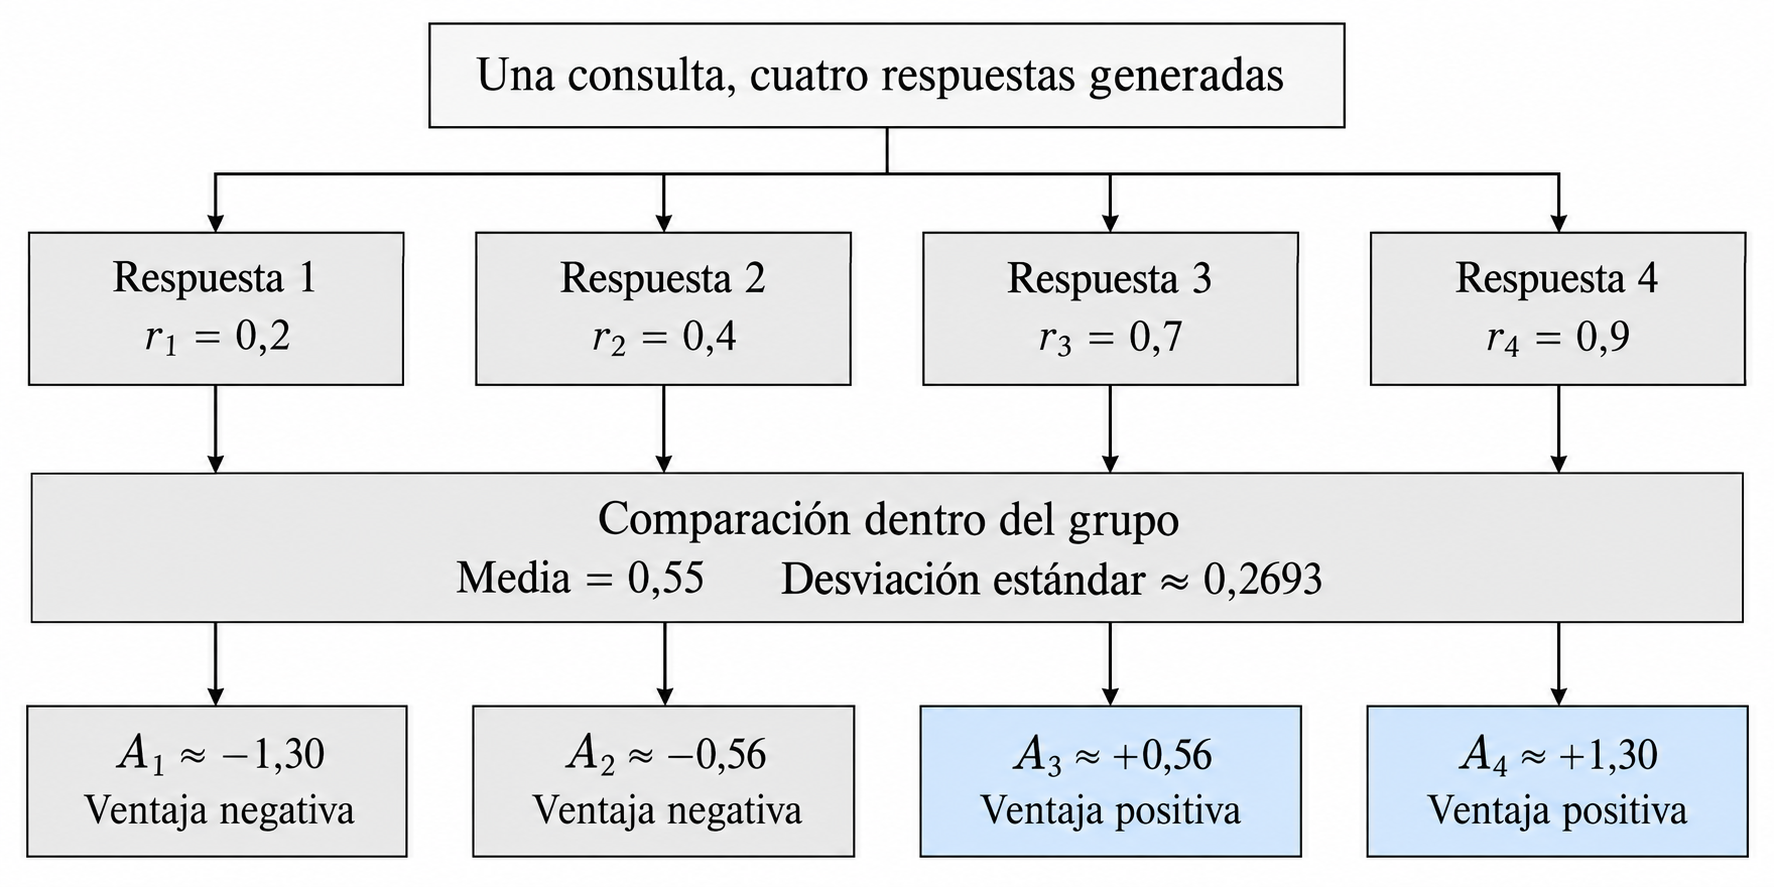
\includegraphics[width=0.95\textwidth]{Figuras/02-marco-teorico/04-ppo-grpo/rl-grpo-grupo.png}
\caption{Ejemplo ilustrativo de comparación de recompensas y ventajas en GRPO.}
\label{fig:grpo-ejemplo}
\end{figure}

Para relacionar esa comparación con la actualización de parámetros, puede escribirse el objetivo de GRPO con recompensa final como
\begin{equation}
\begin{aligned}
J_{\mathrm{GRPO}}(\theta)
&=\mathbb{E}_{x,\{y_i\}\sim\pi_{\mathrm{old}}}\left[
\frac{1}{G}\sum_{i=1}^{G}\frac{1}{T_i}\sum_{t=1}^{T_i}
\left(C_{i,t}(\theta)-\beta D_{i,t}(\theta)\right)\right],\\
C_{i,t}(\theta)
&=\min\left(\rho_{i,t}(\theta)A_i,
\operatorname{clip}(\rho_{i,t}(\theta),1-\epsilon_c,1+\epsilon_c)A_i\right),\\
\rho_{i,t}(\theta)
&=\frac{\pi_\theta(y_{i,t}\mid x,y_{i,<t})}
{\pi_{\mathrm{old}}(y_{i,t}\mid x,y_{i,<t})}.
\end{aligned}
\label{eq:objetivo-grpo}
\end{equation}
En esta expresión, las consultas se extraen de $\mathcal{D}$ y las respuestas se generan con la política de recolección, mientras que $T_i$ es la longitud de la respuesta $i$ y $D_{i,t}$ representa la divergencia respecto de la política de referencia en el contexto del token $t$. El término $C_{i,t}$ combina la razón de probabilidades con la ventaja y el recorte de PPO, mientras que $\beta D_{i,t}$ penaliza la desviación respecto de la referencia~\cite{shao2024deepseekmath}. Por lo tanto, maximizar este objetivo favorece los tokens de respuestas con mejor recompensa relativa, sujeto a esos mecanismos de control, y la pérdida utilizada para minimizar mediante descenso de gradiente puede definirse como $\mathcal{L}_{\mathrm{GRPO}}=-J_{\mathrm{GRPO}}$. La división por $T_i$ da el mismo peso total a cada respuesta antes de promediar el grupo, una elección que puede cambiar en otras variantes.

Cuando se utiliza una recompensa final, la ventaja de la respuesta puede aplicarse a sus tokens durante la actualización, aunque la formulación también contempla señales de proceso y variantes posteriores modifican la normalización y la ponderación por longitud~\cite{shao2024deepseekmath,deepseek2025r1}. En consecuencia, documentar que se utilizó GRPO no basta para reproducir una corrida, sino que deben precisarse su variante, la recompensa y las decisiones de implementación. Además, $G$ indica cuántas respuestas se generan por consulta y debe distinguirse del tamaño del microbatch y de la acumulación de gradientes, definidos en la sección \ref{sec:sft-actualizacion}.

%
%
\section{Rúbricas y modelos de lenguaje como jueces}
\label{sec:marco-rubricas}
En las tareas abiertas, una rúbrica descompone la evaluación en criterios que describen contenidos esperados, restricciones y errores relevantes. Cada criterio puede asociarse con un peso para combinar sus decisiones en una recompensa, permitiendo distinguir respuestas parcialmente satisfactorias. Rubicon estudia esta forma de supervisión en tareas abiertas, mientras que ARES genera preguntas, respuestas y rúbricas a partir de documentos~\cite{huang2025rubicon,li2026ares}.

Rubrics as Rewards (RaR) utiliza rúbricas específicas por consulta como señal de recompensa para entrenar mediante GRPO. Su construcción toma respuestas de referencia como fuente de supervisión y organiza los criterios para que puedan evaluarse individualmente. El trabajo estudia una agregación explícita, que combina decisiones de cumplimiento mediante sus pesos, y una agregación implícita, en la que el juez recibe la rúbrica y produce una puntuación global~\cite{gunjal2025rar}. Esta distinción permite estudiar por separado el contenido de los criterios y la forma en que sus evaluaciones se convierten en recompensa.

\subsection{Evaluación por criterios y ayudas durante la generación}
\label{sec:marco-jueces}
Un modelo de lenguaje puede actuar como juez al recibir la consulta, la respuesta generada y los criterios que debe comprobar. En una evaluación binaria por criterio, sus decisiones indican qué condiciones se cumplen y luego se agregan según sus pesos. A diferencia de una coincidencia literal, esta evaluación permite examinar formulaciones equivalentes, aunque su resultado depende de las instrucciones y de la interpretación del modelo evaluador~\cite{arora2025healthbench,zhou2026ruscarl}.

La rúbrica también puede intervenir en la generación al mostrar parte de sus criterios como ayudas. RuscaRL utiliza distintos niveles de asistencia y reduce su presencia durante el entrenamiento, manteniendo los criterios completos para evaluar las respuestas~\cite{zhou2026ruscarl}. Por ello, conviene distinguir la información visible para el modelo de la que utiliza el juez, así como la recompensa de entrenamiento de la evaluación externa.

\subsection{Limitaciones y evaluación del aprendizaje obtenido}
\label{sec:limites-rl}
La recompensa representa una aproximación al objetivo que se busca mejorar, por lo que maximizarla puede favorecer comportamientos que aprovechen errores del evaluador sin aumentar la calidad de las respuestas. Este fenómeno suele denominarse reward hacking, mientras que la sobreoptimización describe el deterioro que puede aparecer al optimizar excesivamente una señal imperfecta. Gao y sus colaboradores estudiaron esta divergencia mediante un entorno sintético con un modelo de recompensa de referencia y otro utilizado como aproximación, mostrando que el aumento de la señal optimizada puede coexistir con un deterioro de la evaluación de referencia~\cite{gao2022overoptimization}.

Para evaluar el aprendizaje obtenido se distingue la recompensa de entrenamiento del desempeño sobre consultas reservadas y de los resultados de un benchmark externo. La primera describe el ajuste a la señal utilizada, mientras que las otras permiten examinar si ese ajuste mejora las respuestas fuera del entrenamiento. Esta comparación requiere datos separados y protocolos consistentes, y debe complementarse con la revisión de errores que la recompensa puede pasar por alto. En el caso clínico, recuperar los conceptos esperados no basta para comprobar la pertinencia ni la seguridad de todas las recomendaciones, por lo que las rúbricas y las respuestas también requieren revisión experta.%
%
\section{Evaluación de la adaptación}
\label{sec:marco-evaluacion}
La evaluación externa examina las respuestas ante consultas distintas de las utilizadas para entrenar y permite estudiar si los cambios se mantienen fuera de la señal de recompensa. Su interpretación requiere identificar el benchmark, las condiciones de generación y el evaluador, además de definir cómo se agregan los criterios.

\subsection{HealthBench y evaluación por conversación}
\label{sec:marco-healthbench}
HealthBench es un benchmark desarrollado por OpenAI para evaluar respuestas médicas abiertas mediante criterios específicos de cada conversación, elaborados por profesionales médicos~\cite{arora2025healthbench}. Además de su versión general, el benchmark incluye las variantes HealthBench Hard y HealthBench Consensus, por lo que es necesario identificar de cuál procede cada evaluación.

El procedimiento conserva la conversación y su identificador, genera una respuesta al último mensaje del usuario y evalúa cada criterio a partir de esa respuesta y del contexto disponible. Las respuestas se guardan antes de calificarlas, mientras que las decisiones del juez y sus explicaciones se almacenan en archivos separados, lo que permite revisar una decisión individual o recalcular las métricas sin volver a generar el texto. Como muestra la figura \ref{fig:protocolo-evaluacion}, la rúbrica de HealthBench se proporciona únicamente al juez, de modo que el modelo evaluado responde sin acceder a esos criterios. Estas rúbricas pertenecen a la evaluación externa y deben distinguirse de las utilizadas como recompensa durante el entrenamiento.

\begin{figure}[htbp]
\centering
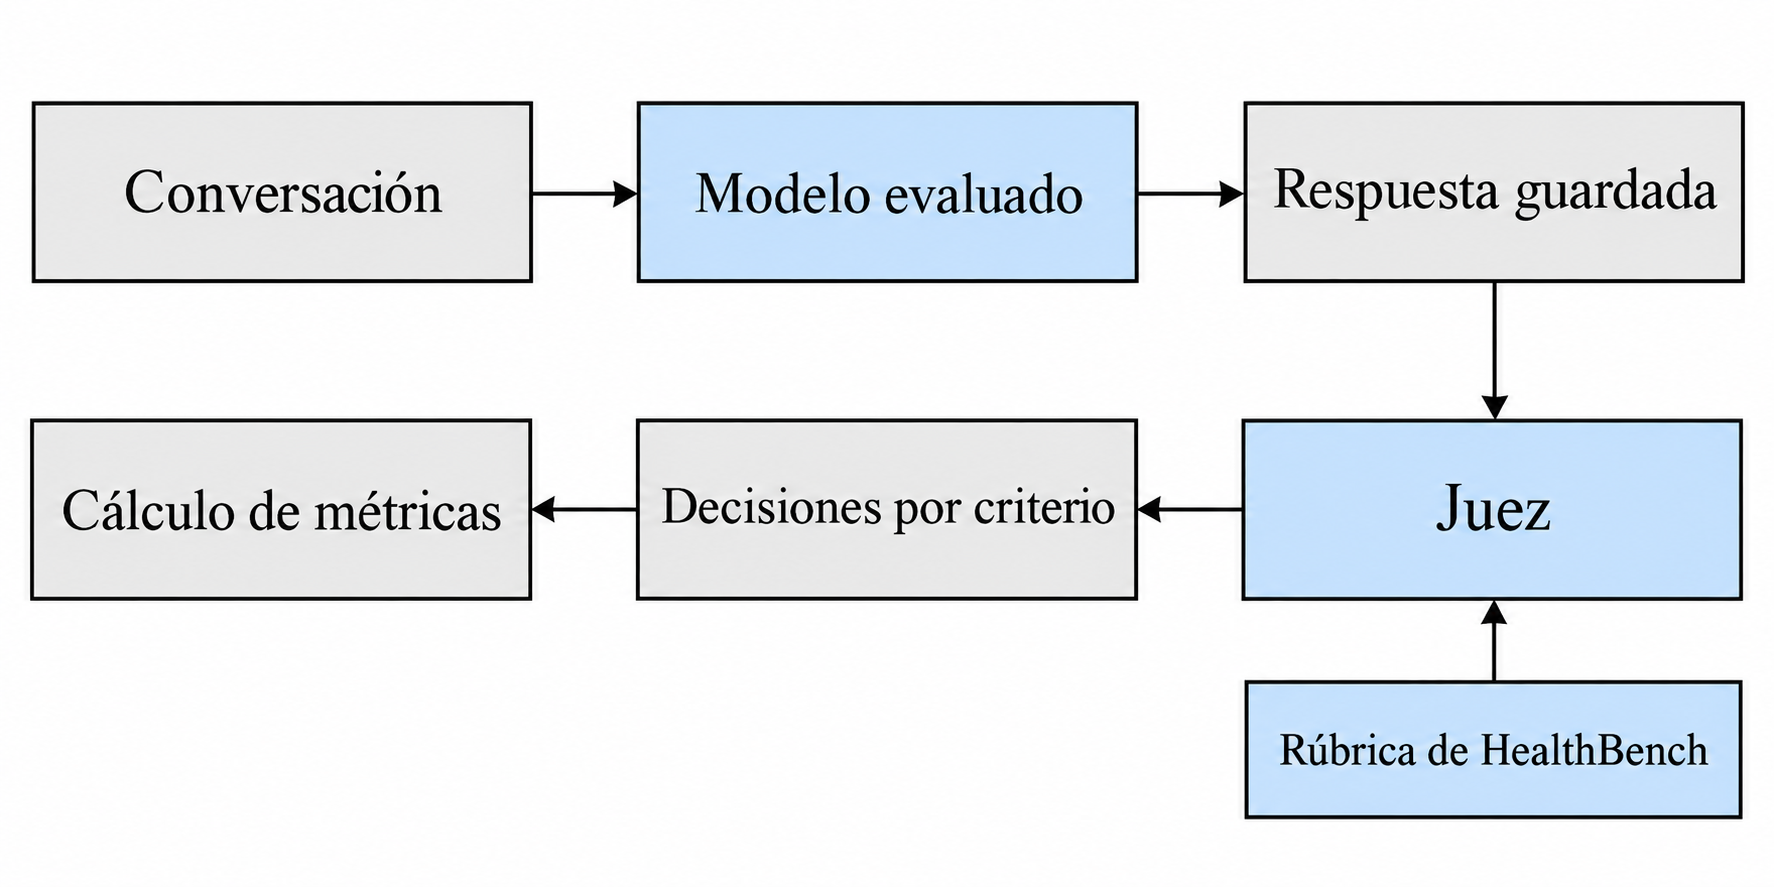
\includegraphics[width=0.95\textwidth]{Figuras/02-marco-teorico/06-evaluacion/evaluacion-protocolo.png}
\caption{Evaluación de respuestas mediante las rúbricas de HealthBench y un modelo juez.}
\label{fig:protocolo-evaluacion}
\end{figure}

Las condiciones concretas de la muestra, la generación y el juez del proyecto se describen en la sección~\ref{sec:protocolo-experimental}.

\subsection{Métricas y comparación de modelos}
\label{sec:evaluacion-metricas}
El puntaje principal combina los criterios cumplidos y sus pesos. Para el caso $i$, sea $p_{ij}$ el peso del criterio $j$ y $m_{ij}\in\{0,1\}$ la decisión de cumplimiento del juez. Si existen puntos positivos disponibles, el valor crudo del caso es
\begin{equation}
s_i=\frac{\sum_{j=1}^{M_i}p_{ij}m_{ij}}
{\sum_{j=1}^{M_i}\max(p_{ij},0)},
\label{eq:healthbench-caso}
\end{equation}
donde $M_i$ es la cantidad de criterios del caso. El numerador incorpora los puntos positivos obtenidos y las penalizaciones activadas, mientras que el denominador representa los puntos positivos disponibles. Por lo tanto, cumplir un criterio de peso negativo resta puntos y puede producir un valor individual negativo.

Para $N$ casos evaluados, el resultado global expresado en porcentaje se calcula como
\begin{equation}
S=100\,\operatorname{clip}\!\left(\overline{s},0,1\right),
\qquad \overline{s}=\frac{1}{N}\sum_{i=1}^{N}s_i.
\label{eq:healthbench-global}
\end{equation}
El orden de estas operaciones sigue el apéndice D de HealthBench y la implementación de simple-evals~\cite{arora2025healthbench,openai2026healthbenchcode}. Primero se promedian los valores crudos y después se recorta el promedio al intervalo indicado, por lo que recortar cada caso antes de promediar corresponde a otro cálculo. En consecuencia, en la formulación de HealthBench un resultado agregado en el extremo inferior puede provenir del recorte de una media neta no positiva y no equivale a que la totalidad de las respuestas sea incorrecta. Por esta razón, el benchmark prevé documentar el comportamiento de las respuestas sin limitarse al puntaje agregado recortado, incorporando desgloses por componentes y el balance de penalizaciones.

El análisis también considera los cinco ejes asociados a los criterios de HealthBench~\cite{arora2025healthbench}, que permiten describir distintos aspectos de una respuesta:

\begingroup
\begin{itemize}
\item \textbf{Precisión:} evalúa la corrección de la información médica y de las recomendaciones, considerando si la respuesta incluye afirmaciones erróneas o presenta como ciertos datos que no están suficientemente respaldados.
\item \textbf{Completitud:} considera si la respuesta cubre la información necesaria para resolver la consulta, incluyendo explicaciones, recomendaciones y advertencias pertinentes, sin omitir aspectos relevantes para el paciente.
\item \textbf{Calidad de comunicación:} examina si la información se presenta de forma clara, comprensible y organizada, con un lenguaje adecuado al interlocutor y un tono que facilite entender las recomendaciones.
\item \textbf{Comprensión del contexto:} valora si la respuesta tiene en cuenta los antecedentes, los síntomas y las circunstancias descritas en la conversación, ajustando sus explicaciones y recomendaciones a la situación particular.
\item \textbf{Seguimiento de instrucciones:} comprueba si la respuesta respeta las solicitudes y restricciones aplicables, como el idioma, el formato o el alcance pedido, manteniendo la atención en lo que se consulta.
\end{itemize}
\endgroup

Para un eje $a$, se calcula el valor del caso utilizando únicamente sus criterios y se incluyen en la agregación los casos con puntos positivos disponibles para ese eje. Si $I_a$ reúne esos casos, el desglose se expresa como
\begin{equation}
s_i^{(a)}=\frac{\sum_{j\in a}p_{ij}m_{ij}}{\sum_{j\in a}\max(p_{ij},0)},
\qquad S^{(a)}=100\,\operatorname{clip}\!\left(
\frac{1}{|I_a|}\sum_{i\in I_a}s_i^{(a)},0,1\right).
\label{eq:healthbench-ejes}
\end{equation}
De este modo, la agregación respeta el peso y la normalización de cada caso, en lugar de promediar directamente porcentajes de criterios cumplidos. En este informe, los desgloses por eje se utilizan para describir el comportamiento de las respuestas bajo el juez local y se presentan separados del puntaje principal.

Como indicadores complementarios, se contabilizan los criterios positivos cumplidos y los criterios negativos activados, expresados como proporciones dentro de cada grupo. Estos conteos no incorporan los pesos, por lo que deben distinguirse de las contribuciones ponderadas al puntaje. Para estudiar ese balance, se separan por caso los términos positivos y negativos del numerador de la ecuación \ref{eq:healthbench-caso}, manteniendo el mismo denominador, y luego se promedian sus contribuciones. Así puede observarse si una mayor cobertura se acompaña de más penalizaciones, sin interpretar todos los criterios negativos como medidas exclusivas de daño clínico.

La comparación pareada utiliza los mismos identificadores para ambos modelos y conserva los valores crudos. Si $s_i^{\mathrm{GRPO}}$ y $s_i^{\mathrm{SFT}}$ son sus respectivos puntajes, se define
\begin{equation}
d_i=s_i^{\mathrm{GRPO}}-s_i^{\mathrm{SFT}},
\qquad \overline{\Delta}=\frac{100}{N}\sum_{i=1}^{N}d_i,
\label{eq:healthbench-pareado}
\end{equation}
con lo que pueden contarse los casos favorables a cada modelo y los empates, además de estimar la diferencia media en puntos porcentuales. El recorte puede ocultar diferencias cuando ambos promedios quedan por debajo de cero o por encima de uno, por lo que también se compara la media de los puntajes crudos. Por otra parte, la longitud de las respuestas, la cobertura de criterios y los errores de evaluación se registran como indicadores descriptivos, sin presentarlos como métricas oficiales adicionales ni como pruebas directas de calidad.

La incertidumbre se estima mediante remuestreo bootstrap de casos. La implementación consultada utiliza 1.000 remuestreos con reemplazo y devuelve la desviación estándar de los puntajes globales recortados, identificada como bootstrap\_std~\cite{openai2026healthbenchcode}. Cuando se informa además un intervalo percentil del 95\%, sus límites se obtienen de los percentiles 2,5 y 97,5 de la distribución remuestreada, por lo que la desviación estándar y el intervalo no constituyen la misma medida. En la comparación entre modelos se remuestrean los mismos casos para ambos y se recalcula la diferencia en cada repetición, conservando así el emparejamiento tanto para la media cruda como para los resultados globales.

El análisis de las métricas se complementa con la revisión de respuestas concretas, especialmente cuando una mayor cobertura se acompaña de más penalizaciones. Examinar esos casos permite distinguir qué información se añadió y qué errores detectó el juez, así como identificar decisiones que requieren revisión experta.%
%

\chapter{Aprendizaje por refuerzo mediante rúbricas extraídas y técnica de scaffolding}
\label{ch:metodo-propuesto}

El método propuesto busca adaptar modelos de lenguaje a dominios abiertos mediante una etapa de post training que combina adaptación supervisada y optimización por refuerzo con rúbricas extraídas de respuestas de referencia. La propuesta parte de que esas respuestas contienen información útil para construir una recompensa, aunque su calidad no pueda comprobarse íntegramente mediante una única regla determinista. En la implementación inicial, se extraen conceptos y expresiones relevantes, se organizan en criterios evaluables y se combinan procedimientos de verificación por código con una evaluación semántica para los casos no resueltos por coincidencia. A su vez, parte de esa información se presenta inicialmente como ayuda y se retira durante el entrenamiento, con el propósito de que el modelo aprenda a responder sin depender de ella.

El procedimiento se estudia mediante una evaluación inicial y un refinamiento posterior apoyado en datos de RaR. Las secciones siguientes distinguen los componentes comunes de las formulaciones propias de cada etapa y reúnen las arquitecturas y la configuración de entrenamiento en la sección~\ref{sec:metodo-entrenamiento}. El capítulo~\ref{ch:evolucion-entrenamiento} presenta los datos y el seguimiento del aprendizaje, mientras que el capítulo~\ref{ch:resultados-adaptacion} reúne la evaluación externa.

\section{Diseño general y separación de los datos}
\label{sec:metodo-datos}
El procedimiento parte de un conjunto de consultas y respuestas de referencia del dominio que se desea abordar. Antes del entrenamiento, los registros se reúnen en un formato común, se eliminan consultas duplicadas y se conserva su procedencia para poder vincular cada rúbrica con la respuesta de la que se extrajo.

En el esquema con una fuente común, el conjunto destinado al aprendizaje se divide en dos particiones: una destinada a la adaptación supervisada y otra reservada para construir las rúbricas y entrenar mediante GRPO. Así, si $\mathcal{D}$ representa el conjunto preparado, la separación se expresa como
\begin{equation}
\mathcal{D}=\mathcal{D}_{\mathrm{SFT}}\cup\mathcal{D}_{\mathrm{reserva}},
\qquad
\mathcal{D}_{\mathrm{SFT}}\cap\mathcal{D}_{\mathrm{reserva}}=\varnothing.
\label{eq:metodo-separacion}
\end{equation}
La primera partición permite adaptar el modelo siguiendo el procedimiento de la sección~\ref{sec:marco-sft}, mientras que las respuestas de la reserva aportan los conceptos utilizados para construir la señal de recompensa. Esta separación evita utilizar las mismas consultas en ambas etapas, aunque no garantiza por sí sola la ausencia de preguntas semánticamente similares.

Cuando se parte de un checkpoint supervisado existente, las fuentes de SFT y de GRPO pueden ser distintas, como ocurre con SFT45k y los datos procedentes de RaR. En ese caso, su independencia debe comprobarse sobre los registros disponibles, sin deducirla únicamente del nombre de las fuentes. Las proporciones de reparto son decisiones experimentales y no una condición fija de la metodología.

Por último, se reservan conjuntos de validación y prueba fuera del aprendizaje, mientras que la evaluación externa utiliza consultas y criterios independientes de los empleados en el entrenamiento, de modo que permite examinar las respuestas sin las ayudas proporcionadas durante GRPO. Las fuentes y las proporciones del particionado se detallan en la sección~\ref{sec:datos-experimentales}, mientras que las arquitecturas y el entrenamiento se reúnen en la sección~\ref{sec:metodo-entrenamiento}.
%
\section{Construcción y refinamiento de rúbricas a partir de referencias}
\label{sec:metodo-criterios}
En la primera etapa, se denominan entidades clave a los conceptos y expresiones relevantes de las respuestas de referencia que se utilizan como unidades de supervisión de la recompensa. El término incluye diagnósticos, localizaciones anatómicas, medicamentos, pruebas y profesionales, además de expresiones que describen acciones recomendadas o la evolución de un problema, de modo que no se restringe a entidades nombradas en sentido estricto. Los siguientes ejemplos presentan una selección real de expresiones de una de las rúbricas del conjunto central, conservando el idioma de los datos originales:

\begingroup
\begin{itemize}
\item \textbf{Boil:} representa un posible diagnóstico mencionado en la respuesta de referencia.
\item \textbf{pubic or groin area:} identifica la localización anatómica del problema descrito.
\item \textbf{resolved on its own:} describe la evolución del problema y su resolución espontánea.
\item \textbf{physical check:} recoge la evaluación física recomendada en la respuesta.
\item \textbf{Surgeon:} identifica al cirujano como uno de los profesionales mencionados.
\item \textbf{GP doctor:} identifica al médico general como otro de los profesionales mencionados.
\end{itemize}
\endgroup

Cada entidad se conserva con un identificador, un peso y una representación léxica que incluye formas normalizadas, lemas, alias y términos considerados esenciales para reconocerla. A partir de esa información se preparan criterios de presencia y, cuando corresponde, criterios de cantidades, postura, relaciones y acciones. Los primeros comprueban valores y unidades asociados a un concepto, mientras que la postura busca distinguir, por ejemplo, una posibilidad de una recomendación. Por su parte, las relaciones se aproximan mediante la presencia de conceptos en una misma oración y su cercanía en tokens, y las acciones se reconocen mediante expresiones compatibles con la familia de acción esperada.

Estas comprobaciones buscan conservar algo más que una lista de palabras, aunque su implementación sigue siendo una aproximación. La aparición de una expresión de posibilidad en una oración no garantiza que modifique el diagnóstico correcto, del mismo modo que dos conceptos cercanos no necesariamente mantienen la relación clínica esperada. Además, la extracción puede conservar fragmentos poco pertinentes, como ocurre en la misma muestra con una referencia a una consulta de seguimiento de pago. Por ello, la selección de entidades también debe revisarse y no puede asumirse que toda expresión extraída constituye un criterio clínico útil.


En la segunda etapa, la construcción parte de las obligaciones explícitas de la pregunta y utiliza la respuesta de referencia para fundamentar los criterios. El objetivo es exigir el contenido necesario para resolver la consulta, sin convertir cada detalle de la referencia en un requisito adicional. Por ello, se identifica si la tarea solicita una respuesta directa, una explicación o varias acciones y se vincula cada criterio con la obligación que evalúa.

Cada criterio evalúa un requisito concreto de la consulta y se vincula con un fragmento de la referencia. También indica qué respuestas equivalentes se aceptan y qué menciones resultarían insuficientes. Por ejemplo, si la consulta pide identificar una sustancia cuyo nivel está elevado, nombrarla sin indicar el sentido del cambio no cubre el requisito completo. El criterio conserva esa relación y su polaridad, y registra la certeza, las condiciones temporales o los parámetros cuando son necesarios para interpretar la respuesta. Si la referencia no permite fundamentar un requisito solicitado, se registra la falta de cobertura.

La generación y la revisión mediante modelos de lenguaje se acompañan de comprobaciones estructurales y de correspondencia con la evidencia. Este control busca mejorar la fidelidad de la rúbrica a la consulta y a la referencia, aunque no constituye una revisión médica de su corrección. Los criterios aceptados se clasifican como esenciales o adicionales y se puntúan con la formulación correspondiente a la segunda etapa, descrita en la sección~\ref{sec:metodo-recompensa}.
%
\section{Evaluación de criterios y formulaciones de recompensa}
\label{sec:metodo-recompensa}
\subsection{Evaluación híbrida y recompensa de la primera etapa}
La evaluación inicial comienza con un procedimiento determinista que normaliza la respuesta y busca las entidades dentro de sus oraciones. Una coincidencia puede obtenerse mediante una expresión exacta o mediante una cobertura suficiente de grupos de términos y anclas, utilizando los lemas y los alias previstos para cada concepto. Este procedimiento reduce el costo de evaluación y permite registrar qué términos respaldan cada detección, aunque puede producir falsos negativos ante paráfrasis y falsos positivos cuando una expresión aparece en un contexto inadecuado.

Para ampliar la cobertura, las entidades no detectadas por código se envían a un juez semántico junto con la consulta, la respuesta generada y la información asociada al criterio. El juez debe señalar si el concepto está presente y aportar un fragmento de evidencia, cuya presencia en una oración de la respuesta se comprueba antes de aceptar la detección. De este modo, la evaluación semántica puede recuperar menciones que el diccionario no reconoce, pero no reemplaza todas las comprobaciones ni revisa automáticamente las coincidencias positivas del código. La verificación del fragmento acredita que la evidencia está en el texto, sin garantizar por sí sola la corrección clínica de la interpretación.

La recompensa combina cinco componentes, cuyos valores se denotan por $E$, $N$, $T$, $B$ y $A$, correspondientes a entidades, cantidades, postura, relaciones y acciones. Como algunos ejemplos no contienen todos los tipos de criterio, los pesos se normalizan entre los componentes disponibles. Si $\mathcal{K}_i$ reúne los componentes activos del ejemplo $i$ y $b_k$ es el presupuesto del componente $k$, se define
\begin{equation}
\alpha_{ik}=\frac{b_k}{\sum_{\ell\in\mathcal{K}_i}b_\ell},
\qquad
R_i(y)=\operatorname{clip}\!\left(
\sum_{k\in\mathcal{K}_i}\alpha_{ik}C_{ik}(y)-P_i(y),-1,1\right),
\label{eq:metodo-recompensa}
\end{equation}
donde $C_{ik}(y)$ representa el valor del componente evaluado sobre la respuesta $y$ y $P_i(y)$ reúne las penalizaciones. Así, la ausencia de criterios numéricos en un ejemplo no se interpreta como un incumplimiento ni reduce automáticamente su recompensa máxima.

Las penalizaciones contemplan respuestas vacías, repetición de secuencias y listas breves de palabras clave, buscando reducir formas de obtener cobertura sin desarrollar una explicación útil. Los presupuestos de los componentes y los valores de las penalizaciones utilizados en el experimento central se detallan en la sección~\ref{sec:protocolo-configuracion}. Estos mecanismos no constituyen una evaluación completa de seguridad clínica, ya que no comprueban de manera general contraindicaciones, daño potencial ni la pertinencia de toda recomendación.


\subsection{Evaluación semántica y recompensa del piloto posterior}
En el piloto de la segunda etapa, el juez evalúa el significado de cada criterio y asigna un estado de cumplimiento, ausencia, contradicción, no aplicabilidad o incertidumbre. La decisión debe estar respaldada por evidencia literal cuando corresponde, y una contradicción aplicable impide considerar satisfecho el criterio. Así, el control por código comprueba la integridad del veredicto y la evidencia, mientras que el juicio sobre el cumplimiento del requisito es semántico; este reparto difiere de la búsqueda léxica seguida de revisión de entidades no detectadas utilizada inicialmente.

Si $\mathcal{A}_i$ es el conjunto de criterios aplicables a la respuesta $y$ del ejemplo $i$, $v_j$ su peso positivo y $s_j(y)$ vale 1 únicamente cuando el criterio está satisfecho, la recompensa del piloto es
\begin{equation}
R_i^{\mathrm{piloto}}(y)=
\frac{\sum_{j\in\mathcal{A}_i}v_j s_j(y)}{\sum_{j\in\mathcal{A}_i}v_j}.
\label{eq:metodo-recompensa-piloto}
\end{equation}
Los criterios esenciales tienen peso 3 y los adicionales peso 1. La ausencia o la contradicción no aportan crédito y no reciben una penalización numérica adicional, mientras que la no aplicabilidad requiere una condición prevista en la rúbrica. Por su parte, la incertidumbre, la evidencia inválida o los veredictos incompletos bloquean el cálculo y la actualización correspondiente, en lugar de convertirse automáticamente en una recompensa nula.

Esta formulación concreta permite estudiar una señal basada en la satisfacción de obligaciones y debe distinguirse de otras variantes de recompensa que se investiguen posteriormente. El contraste con RaR requiere examinar tanto la construcción de los criterios como su agregación~\cite{gunjal2025rar}; utilizar preguntas y respuestas de ese trabajo no implica conservar su rúbrica, sus pesos ni su protocolo experimental.
%
\section{Retirada progresiva de ayudas durante el entrenamiento}
\label{sec:metodo-ayudas}
La retirada progresiva de ayudas, denominada scaffold, presenta al modelo parte de las entidades esperadas junto con la consulta al comienzo del entrenamiento. Su propósito es facilitar la incorporación del contenido del dominio y aumentar después la exigencia de recuperación autónoma, por lo que las entidades visibles se reducen a medida que avanza el calendario. La rúbrica completa permanece disponible para evaluar la respuesta, aunque el modelo recibe únicamente la fracción de conceptos habilitada para esa presentación.

El calendario establece una fracción de entidades visibles para cada etapa, que se reduce hasta llegar a consultas sin ayudas. Para ello, se asigna un orden a las entidades de cada ejemplo y se conservan subconjuntos cada vez menores, manteniendo la rúbrica completa para evaluar todas las respuestas. La duración del calendario y las reglas de selección empleadas en el experimento central se detallan en la sección~\ref{sec:protocolo-configuracion}.

La figura~\ref{fig:scaffolding-etapas} ilustra este mecanismo con el calendario definido en el diseño posterior V29. En esa implementación, un modelo de lenguaje genera ayudas breves a partir de los criterios y de la evidencia de la respuesta de referencia, y una revisión mediante LLM comprueba su correspondencia con esas fuentes antes de incorporarlas al entrenamiento. Las ayudas aceptadas se ordenan de manera determinista y, en cada etapa, se conserva la cantidad correspondiente a la tasa de retención, redondeada hacia arriba. Por ejemplo, cuatro ayudas dan lugar a subconjuntos de cuatro, tres, dos, una y ninguna ayuda para las tasas de 100\%, 75\%, 50\%, 25\% y 0\%, respectivamente. Este ejemplo representa el diseño de V29; el calendario del experimento central evaluado en este informe se especifica en la sección~\ref{sec:protocolo-configuracion}.

\begin{figure}[htbp]
\centering
\begingroup
\singlespacing
\shorthandoff{<>}
\definecolor{scaffoldink}{HTML}{253F53}
\definecolor{scaffoldline}{HTML}{658AA8}
\definecolor{scaffoldcream}{HTML}{F7FAFC}
\definecolor{scaffoldpeach}{HTML}{C7DCEC}
\definecolor{scaffoldsand}{HTML}{DBE7F0}
\definecolor{scaffoldshadow}{HTML}{D6E0E8}
\resizebox{\textwidth}{!}{%
\begin{tikzpicture}[>=Stealth,
 base/.style={rounded corners=9pt,draw=scaffoldline,line width=.9pt,fill=scaffoldcream},
 title/.style={align=center,text=scaffoldink,font=\sffamily\small\bfseries,inner sep=2pt},
 body/.style={align=center,text=scaffoldink,font=\sffamily\small,inner sep=0pt},
 branch/.style={draw=scaffoldline,line width=1.3pt,rounded corners=8pt,line cap=round,line join=round}]
% Tarjetas superiores: cabecera y cuerpo, con sombra discreta.
\fill[scaffoldshadow,rounded corners=9pt] (4.04,4.23) rectangle (9.24,5.71);
\draw[base] (4.12,4.32) rectangle (9.32,5.8);
\draw[draw=scaffoldline,fill=scaffoldpeach,rounded corners=6pt,line width=.8pt]
 (4.3,5.15) rectangle (9.14,5.59);
\node[title] at (6.72,5.37) {LLM};
\node[body] at (6.72,4.73) {Generación de rúbricas};
\fill[scaffoldshadow,rounded corners=9pt] (4.04,2.48) rectangle (9.24,3.61);
\draw[base] (4.12,2.57) rectangle (9.32,3.7);
\draw[draw=scaffoldline,fill=scaffoldsand,rounded corners=6pt,line width=.8pt]
 (4.3,2.88) rectangle (9.14,3.39);
\node[title] at (6.72,3.135) {Entrenamiento con GRPO};
\draw[branch] (6.72,4.32) -- (6.72,3.7);
% Una única línea conecta GRPO con todas las etapas.
\draw[branch] (6.72,2.57) -- (6.72,1.92);
\draw[branch] (0,1.12) -- (0,1.64) -- (13.44,1.64) -- (13.44,1.12);
\foreach \x in {3.36,6.72,10.08} {
 \draw[branch] (\x,1.64) -- (\x,1.12);
}
\draw[branch] (6.72,1.92) -- (6.72,1.64);
% Etapas con cabeceras de tonos azules y porcentajes destacados.
\foreach \x/\n/\pct/\tone in {0/1/100/scaffoldpeach,3.36/2/75/scaffoldpeach!75!scaffoldsand,6.72/3/50/scaffoldsand,10.08/4/25/scaffoldsand!65!scaffoldcream,13.44/5/0/scaffoldsand!35!scaffoldcream} {
 \fill[scaffoldshadow,rounded corners=9pt] (\x-1.5,-1.76) rectangle (\x+1.34,1.03);
 \draw[base] (\x-1.42,-1.67) rectangle (\x+1.42,1.12);
 \draw[draw=scaffoldline,fill=\tone,rounded corners=6pt,line width=.8pt]
 (\x-1.25,.46) rectangle (\x+1.25,.91);
 \node[title] at (\x,.685) {Etapa \n};
 \node[body,font=\normalfont\large] at (\x,-.13) {\pct\%};
 \node[body] at (\x,-1.02) {de entidades\\en el input};
}
\end{tikzpicture}%
}
\endgroup

\caption{Retirada progresiva de ayudas en cinco etapas de entrenamiento.}
\label{fig:scaffolding-etapas}
\end{figure}

En la formulación inicial, la recompensa distingue entre conceptos visibles y ocultos para dar mayor peso a la recuperación sin ayuda. Si $w_e$ es el peso base de la entidad $e$, $m_e$ su puntuación de detección y $\lambda_e$ es un multiplicador que toma un valor mayor para las entidades ocultas que para las visibles, el componente de entidades se calcula como
\begin{equation}
E_i(y)=\min\!\left(1,
\frac{\sum_e w_e\lambda_e m_e}{\sum_e w_e\lambda_e}
+\eta\,\frac{H_i^{\mathrm{rec}}}{H_i}\right),
\label{eq:metodo-entidades-ocultas}
\end{equation}
donde $H_i$ es la cantidad de entidades ocultas, $H_i^{\mathrm{rec}}$ la cantidad recuperada y $\eta$ controla la bonificación por su recuperación. El término adicional se toma como cero cuando no hay entidades ocultas. Esta formulación añade una bonificación máxima de $\eta$ al componente, que luego se combina con los restantes mediante la ecuación~\ref{eq:metodo-recompensa}.

El mecanismo busca que recuperar información no presentada resulte más valioso que repetir las ayudas, aunque su efecto depende de la composición de cada ejemplo. Cuando todas las entidades están ocultas, el multiplicador común se cancela en el cociente ponderado y la diferencia adicional procede de la bonificación. Por ello, la asimetría tiene un efecto relativo especialmente en las etapas con entidades visibles y ocultas. Asimismo, las respuestas generadas con ayudas deben distinguirse de las producidas sin ellas al analizar el comportamiento del modelo.


En el piloto posterior, las ayudas se vinculan a los criterios y a la evidencia de referencia y se retiran siguiendo el calendario de cinco etapas de la figura~\ref{fig:scaffolding-etapas}. Las tasas representan retención nominal: el redondeo hacia arriba puede producir la misma cantidad de ayudas en etapas consecutivas cuando hay pocas disponibles. La validación se realiza sin ayudas, mientras que el juez utiliza la rúbrica completa y no recibe las ayudas visibles en el prompt del modelo. A diferencia de la formulación inicial, la recompensa de la ecuación~\ref{eq:metodo-recompensa-piloto} conserva los pesos de los criterios durante las etapas y no aplica el multiplicador por entidades ocultas de la ecuación~\ref{eq:metodo-entidades-ocultas}.
%
\section{Integración de las rúbricas y las ayudas con GRPO}
\label{sec:metodo-integracion}
Una vez preparado el conjunto con sus rúbricas y máscaras de visibilidad, el modelo adaptado genera un grupo de respuestas para cada consulta y cada respuesta recibe una recompensa mediante el procedimiento anterior. Esos valores alimentan la comparación relativa descrita en la sección \ref{sec:grpo}, de modo que GRPO actualiza la política utilizando las diferencias dentro del grupo~\cite{shao2024deepseekmath}. La propuesta conserva ese mecanismo de optimización y modifica principalmente la construcción de la señal y las ayudas disponibles durante las distintas etapas.

Durante el entrenamiento se registran las respuestas, las decisiones de presencia, la evidencia semántica, los valores de cada componente y las penalizaciones. Estos registros permiten analizar si una variación de la recompensa procede de recuperar contenido, de cambios en las ayudas o de evitar determinadas formas de respuesta. La configuración utilizada para aplicar este procedimiento se describe en la sección~\ref{sec:protocolo-configuracion}, mientras que la evaluación externa emplea criterios independientes de los utilizados para entrenar.


La misma secuencia de generación, evaluación y actualización se mantiene en la segunda etapa, utilizando las rúbricas refinadas y la recompensa del piloto. En consecuencia, los cambios en la construcción de criterios y en su puntuación pueden estudiarse dentro del procedimiento común, conservando una referencia KL correspondiente al modelo adaptado mediante SFT. Las configuraciones de ambas etapas se detallan en la sección~\ref{sec:metodo-entrenamiento}.
%
\section{Entrenamiento}
\label{sec:metodo-entrenamiento}
\label{sec:metodo-evolucion}
Las pruebas iniciales utilizan Qwen2.5-7B, mientras que la comparación con el trabajo externo parte de Qwen2.5-3B SFT45k.

\subsection{Elección de las arquitecturas}
\label{sec:metodo-arquitecturas}
Se utilizan dos tamaños de la familia Qwen2.5, de 7B y 3B parámetros~\cite{qwen2024qwen25}. El alcance de las comparaciones se establece en la sección~\ref{sec:resultados-modelos}.

En la primera etapa, Qwen2.5-7B Base proporciona el punto de partida para obtener el modelo SFT-90 y estudiar después su adaptación con GRPO. Durante GRPO se actualizan los parámetros de LoRA asociados a las proyecciones de atención y del bloque de transformación, mientras que los embeddings y la cabeza de salida guardados con el adaptador se congelan en esta etapa.

Para estudiar las nuevas rúbricas y recompensas se utiliza Qwen2.5-3B, buscando reducir el costo de los experimentos. Se parte del checkpoint SFT45k adaptado mediante QLoRA y actualización de embeddings. El adaptador supervisado se fusiona con el modelo base y se conservan los embeddings adaptados; a partir de esa misma versión se construyen la política entrenable y la referencia congelada utilizada para la regularización KL. Durante GRPO se incorporan nuevos adaptadores LoRA y se entrenan también los embeddings, manteniendo el enlace con la cabeza de salida cuando corresponde.

\subsection{Configuración de entrenamiento}
\label{sec:metodo-configuracion}
\label{sec:protocolo-configuracion}
\subsubsection{Pruebas del método de adaptación a dominios abiertos}
En la primera etapa, la adaptación supervisada utiliza la partición del 90\% de las consultas y respuestas preparadas, mientras que la reserva aporta los ejemplos para las rúbricas y GRPO. El entrenamiento posterior parte de SFT-90 y actualiza adaptadores LoRA de rango 64 y escala 16. Las fuentes y el particionado se detallan en la sección~\ref{sec:protocolo-primera-etapa}.

El entrenamiento utiliza 16 generaciones por consulta, una tasa de aprendizaje de $5\times10^{-6}$, un coeficiente de regularización KL de 0,04 y un máximo de 250 tokens nuevos por respuesta, con temperatura 0,7 y top\_p de 0,9. Cada una de las 500 consultas se presenta en diez etapas de ayudas, formando un conjunto de 5.000 entradas que el entrenador recorre una vez.

Los pesos iniciales de los componentes de recompensa son 0,55 para entidades, 0,20 para cantidades, 0,15 para postura, 0,05 para relaciones y 0,05 para acciones, normalizados entre los componentes activos de cada ejemplo según la ecuación~\ref{eq:metodo-recompensa}. Las penalizaciones corresponden a respuestas vacías, repetición de secuencias de tres tokens y listas breves de palabras clave, con un valor de 1 para las respuestas vacías y máximos de 0,10 y 0,05 para las otras dos, respectivamente.

Durante las primeras nueve etapas, todas pueden recibir ayudas, pero la proporción de entidades conservadas como ayuda desciende del 100\% al 20\% en pasos de diez puntos porcentuales, mientras que en la décima etapa no se muestra ninguna entidad. La cantidad visible se obtiene redondeando hacia arriba y conservando al menos una entidad cuando existe asistencia, de modo que la proporción efectiva depende de cuántos conceptos contenga cada rúbrica. Además, la selección utiliza un orden determinista que permite que las ayudas de una etapa posterior formen un subconjunto de las anteriores.

En la ecuación~\ref{eq:metodo-entidades-ocultas}, el multiplicador $\lambda_e$ vale 1 para las entidades visibles y 2,5 para las ocultas, mientras que la bonificación máxima por recuperación se fija en $\eta=0{,}05$.

\subsubsection{Comparación con un trabajo externo}
El entrenamiento supervisado de SFT45k comprende dos épocas sobre 45.000 muestras. El entrenamiento con GRPO parte de este checkpoint y utiliza preguntas y respuestas procedentes de RaR, cuyos conjuntos de entrenamiento y validación se describen en la sección~\ref{sec:protocolo-segunda-etapa}.

El piloto configura nuevos adaptadores LoRA de rango 16 y escala 32, con una tasa de aprendizaje de $2\times10^{-6}$, mientras que los embeddings se actualizan con una tasa de $2\times10^{-7}$. Se generan 16 respuestas por consulta con temperatura 0,7, top\_p de 0,9 y un máximo de 1.024 tokens nuevos. El coeficiente de regularización KL es 0,04 y el objetivo utiliza normalización BNPO, con una única actualización por grupo. La generación se organiza en microbatches de ocho respuestas y el cálculo de gradientes en cuatro microbatches de cuatro respuestas.

El calendario del piloto recorre las consultas en cinco etapas con proporciones de ayudas de 100\%, 75\%, 50\%, 25\% y 0\%, utilizando el orden fijo y el redondeo hacia arriba descritos en la sección~\ref{sec:metodo-ayudas}. La validación se realiza sin ayudas antes del entrenamiento y al finalizar cada etapa. La puntuación sigue la ecuación~\ref{eq:metodo-recompensa-piloto}, con pesos de 3 para criterios esenciales y 1 para adicionales, y permanece independiente de las ayudas visibles para el modelo.

%
\section{Métricas de evaluación}
\label{sec:metodo-metricas}
La pérdida supervisada permite seguir el ajuste a las respuestas de referencia, mientras que la recompensa de GRPO mide el cumplimiento de las rúbricas de entrenamiento. La evaluación en HealthBench examina después las respuestas con criterios externos al aprendizaje.

\subsection{Seguimiento del ajuste supervisado}
\label{sec:metricas-sft}
Durante SFT se registra la pérdida de entrenamiento sobre los tokens supervisados, definida en la ecuación~\ref{eq:sft-mascara}. Su descenso indica que el modelo asigna mayor probabilidad a las respuestas de referencia. La pérdida de validación aplica el mismo cálculo a ejemplos separados, sin actualizar parámetros, para seguir el ajuste fuera de los datos utilizados en cada paso.

Los registros también incluyen la tasa de aprendizaje y la norma del gradiente. En SFT45k se contabilizan los tokens supervisados y su velocidad de procesamiento, lo que permite relacionar cada actualización con el volumen de texto aprendido y el tiempo empleado. Estos valores describen el comportamiento del entrenamiento; la calidad de las respuestas generadas se examina mediante la evaluación posterior.

\subsection{Seguimiento del entrenamiento con GRPO}
\label{sec:metricas-grpo}
La medida principal es la recompensa media de las respuestas generadas para cada consulta. Junto con ella se registra su desviación estándar dentro del grupo, porque las diferencias entre respuestas determinan las ventajas utilizadas por GRPO. En el piloto posterior también se identifica la frecuencia de grupos con recompensas idénticas. Para visualizar la tendencia se conserva una media móvil exponencial, además de los valores sin suavizar.

La pérdida de optimización, la divergencia KL respecto de la referencia y la norma del gradiente permiten seguir las actualizaciones. También se registra la longitud de las respuestas; en el piloto se añade la proporción de salidas que alcanzan el límite de generación. Las métricas se relacionan con la etapa y con la cantidad de ayudas visibles, ya que una recompensa obtenida con asistencia completa no tiene la misma dificultad que una obtenida sin ayudas.

En el piloto posterior se registra por separado la proporción de criterios esenciales y adicionales satisfechos, junto con los estados asignados por el juez. La validación utiliza consultas sin ayudas y registra la recompensa media, su dispersión y la proporción de respuestas truncadas, antes del entrenamiento y al terminar cada etapa. Esta evaluación permite observar el comportamiento sin asistencia mientras cambia la cantidad de ayudas del conjunto de entrenamiento.

\subsection{Evaluación externa en HealthBench}
\label{sec:metricas-benchmark}
HealthBench combina los criterios cumplidos y sus pesos en una puntuación por conversación. El resultado global promedia esos valores y aplica el recorte definido en la ecuación~\ref{eq:healthbench-global}~\cite{arora2025healthbench,openai2026healthbenchcode}. El procedimiento se desarrolla en la sección~\ref{sec:marco-evaluacion}, mientras que las condiciones del juez y de generación del proyecto se detallan en la sección~\ref{sec:protocolo-experimental}.

Para analizar la primera etapa se presentan desgloses de precisión, calidad de comunicación, comprensión del contexto y seguimiento de instrucciones, calculados según la ecuación~\ref{eq:healthbench-ejes}. También se cuentan los criterios positivos cumplidos y los negativos activados, con sus respectivas proporciones. Estos conteos permiten reconocer si una mayor cobertura se acompaña de más errores, aunque no incorporan los pesos utilizados en la puntuación del benchmark.

La comparación entre SFT-90 y SFT-90 + GRPO utiliza los mismos casos y expresa las diferencias entre ejes en puntos porcentuales. Los fragmentos de respuestas del análisis cualitativo ayudan a interpretar qué cambios de contenido acompañan esas diferencias. Los resultados corresponden a la evaluación con el juez local utilizado en el proyecto.



\chapter{Evolución del aprendizaje durante la adaptación}
\label{ch:evolucion-entrenamiento}
El seguimiento del entrenamiento permite observar cómo cambian las pérdidas y las recompensas antes de evaluar las respuestas en un benchmark. Este capítulo reúne los datos de las dos etapas, analiza los historiales disponibles de SFT y GRPO y relaciona su evolución con la retirada de ayudas. Las arquitecturas y los hiperparámetros se describen en la sección~\ref{sec:metodo-entrenamiento}.

\section{Datos y particiones para las dos etapas}
\label{sec:datos-experimentales}
\subsection{Pruebas del método de adaptación a dominios abiertos}
\label{sec:protocolo-primera-etapa}
La aplicación estudiada utiliza consultas médicas abiertas de HealthCareMagic e iCliniq, recopiladas en ChatDoctor~\cite{li2023chatdoctor}. Sus autores describen un filtrado automático de conversaciones demasiado breves y una revisión manual de respuestas con errores en HealthCareMagic, junto con la eliminación de información identificatoria y la corrección gramatical. Para iCliniq, señalan una selección aleatoria estratificada por especialidades y la eliminación de información identificatoria. Estas medidas respaldan la procedencia y la curación de los datos, aunque no acreditan una certificación clínica individual de todas las respuestas, por lo que en este trabajo se reutilizan como referencias de supervisión sin una validación clínica adicional de las rúbricas derivadas.

La preparación reúne ambas fuentes en un esquema común de consulta, respuesta y procedencia, elimina consultas duplicadas entre las fuentes y ordena los registros mediante una mezcla reproducible con semilla 42. Sobre esa lista se reserva el 90\% para SFT y el 10\% restante para la extracción de criterios y el entrenamiento posterior, siguiendo la separación definida en la ecuación~\ref{eq:metodo-separacion}. El código conserva el índice global de cada registro y verifica que las particiones no compartan índices, aunque esta comprobación no permite descartar coincidencias con los datos de preentrenamiento del modelo.

El conjunto central de GRPO contiene 500 consultas con sus criterios compilados y conserva los índices que permiten vincularlas con la reserva. Este conjunto pertenece al entrenamiento y es independiente de la muestra de HealthBench utilizada para la evaluación externa.


\subsection{Comparación con un trabajo externo}
\label{sec:protocolo-segunda-etapa}
\subsubsection{Checkpoint supervisado y procedencia de sus datos}
El conjunto de entrenamiento del checkpoint SFT45k reúne 45.000 muestras de cuatro fuentes. La tabla~\ref{tab:sft45k-fuentes} presenta su composición, mientras que el modelo y su adaptación se describen en la sección~\ref{sec:metodo-arquitecturas}.

\begin{table}[htbp]
\centering
\caption{Fuentes del entrenamiento supervisado SFT45k.}
\label{tab:sft45k-fuentes}
\begin{tabular}{cc}
\toprule
Fuente & Muestras de entrenamiento \\
\midrule
MuSeR & 27.000 \\
HealthCareMagic & 10.515 \\
MedQuad & 6.750 \\
iCliniq & 735 \\
\midrule
Total & 45.000 \\
\bottomrule
\end{tabular}
\end{table}

Estas fuentes pertenecen a SFT. Las preguntas y respuestas procedentes de RaR se incorporan después para construir las rúbricas y preparar GRPO, por lo que no deben confundirse con la composición de SFT45k. La comprobación de coincidencias entre las fuentes debe realizarse sobre los registros efectivos antes de interpretar su separación como independencia experimental.

\subsubsection{Datos del piloto}
El piloto utiliza un subconjunto de 300 muestras de entrenamiento y 50 de validación, cada una con su rúbrica y su revisión, procedentes de los datos de RaR.

La arquitectura y la configuración de entrenamiento del piloto se detallan en la sección~\ref{sec:metodo-entrenamiento}, mientras que la composición de SFT45k y el subconjunto de RaR definen las fuentes utilizadas en esta etapa.


\subsection{Experimento final previsto}
\label{sec:protocolo-final-previsto}
El diseño final contempla reservar validación y prueba fuera del aprendizaje y dividir el conjunto restante en un 50\% para SFT y un 50\% para GRPO. Las rúbricas se extraerán de las respuestas de referencia de esta segunda mitad. Esta configuración es una propuesta y debe distinguirse tanto del checkpoint SFT45k como del piloto de 300 muestras de entrenamiento y 50 de validación. Su ejecución y evaluación permanecen pendientes, y el reparto propuesto no se presenta como una reproducción del protocolo de RaR.

\section{Evolución de los modelos durante el entrenamiento}
\label{sec:evolucion-modelos}
\subsection{Ajuste supervisado de la primera etapa}
El historial de SFT conservado junto al adaptador de la primera etapa registra cinco épocas de entrenamiento. La figura~\ref{fig:sft-inicial-curvas} muestra la pérdida de entrenamiento y las evaluaciones realizadas al terminar cada época. Para hacer visible la tendencia, la curva de entrenamiento utiliza una media móvil de 25 registros; los valores individuales se mantienen en un tono más claro.

\begin{figure}[htbp]
\centering
\begingroup
\singlespacing
\shorthandoff{<>}
\begin{tikzpicture}
\begin{axis}[width=.98\textwidth,height=6.4cm,
 xlabel={Épocas},ylabel={Pérdida},
 grid=major,grid style={gray!15},axis lines=left,
 tick label style={font=\footnotesize},label style={font=\small},
 legend style={font=\footnotesize,draw=none,at={(.98,.98)},anchor=north east,fill=white},
 scaled ticks=false]
\addplot[color=blue!18,line width=.3pt,forget plot] table[x=x,y=loss] {Figuras/04-entrenamiento/sft-inicial-train.dat};
\addplot[color={rgb,255:red,53;green,95;blue,128},line width=1.1pt] table[x=x,y=smooth] {Figuras/04-entrenamiento/sft-inicial-train.dat};
\addlegendentry{Entrenamiento (media móvil)}
\addplot[color={rgb,255:red,179;green,104;blue,62},mark=*,mark size=1.5pt,line width=1pt] table[x=x,y=loss] {Figuras/04-entrenamiento/sft-inicial-validation.dat};
\addlegendentry{Validación}
\end{axis}
\end{tikzpicture}
\endgroup

\caption{Pérdidas de entrenamiento y validación del SFT inicial.}
\label{fig:sft-inicial-curvas}
\end{figure}

La pérdida de validación desciende de 1,873 al finalizar la primera época a 1,812 en la tercera, y después aumenta hasta 1,884 en la quinta. En cambio, la pérdida de entrenamiento continúa descendiendo. Esta separación muestra que prolongar el ajuste mejora la reproducción de los ejemplos de entrenamiento sin producir la misma evolución en el conjunto de validación.

\subsection{Entrenamiento posterior con GRPO}
El modelo adaptado mediante SFT se utiliza después para generar y evaluar grupos de respuestas sobre las consultas reservadas. Las diez etapas modifican la cantidad de entidades disponibles como ayuda, con la configuración descrita en la sección~\ref{sec:metodo-configuracion}. Para analizar su evolución, las curvas de recompensa y KL deben conservar esa referencia temporal y distinguir los tramos asistidos del tramo final sin ayudas.

Las respuestas del modelo obtenido se evalúan después en HealthBench, con los resultados presentados en la sección~\ref{sec:evaluacion-healthbench}.

\section{Refinamiento del entrenamiento a partir de RaR}
\label{sec:refinamiento-entrenamiento-rar}
\subsection{Adaptación supervisada de Qwen2.5-3B}
El registro de SFT45k contiene 2.870 actualizaciones y 20 evaluaciones de validación. La pérdida de validación pasa de 1,195 en la primera evaluación, realizada en el paso 150, a 1,021 al terminar el entrenamiento. La figura~\ref{fig:sft45k-curvas} muestra ese recorrido con el mismo suavizado de 25 registros utilizado para visualizar la pérdida de entrenamiento del SFT inicial.

\begin{figure}[htbp]
\centering
\begingroup
\singlespacing
\shorthandoff{<>}
\begin{tikzpicture}
\begin{axis}[width=.98\textwidth,height=6.4cm,
 xlabel={Pasos de optimización},ylabel={Pérdida},
 grid=major,grid style={gray!15},axis lines=left,
 tick label style={font=\footnotesize},label style={font=\small},
 legend style={font=\footnotesize,draw=none,at={(.98,.98)},anchor=north east,fill=white},
 scaled ticks=false,xtick={0,500,1000,1500,2000,2500},
 xticklabel style={/pgf/number format/1000 sep={.}}]
\addplot[color=blue!18,line width=.3pt,forget plot] table[x=x,y=loss] {Figuras/04-entrenamiento/sft45k-train.dat};
\addplot[color={rgb,255:red,53;green,95;blue,128},line width=1.1pt] table[x=x,y=smooth] {Figuras/04-entrenamiento/sft45k-train.dat};
\addlegendentry{Entrenamiento (media móvil)}
\addplot[color={rgb,255:red,179;green,104;blue,62},mark=*,mark size=1.5pt,line width=1pt] table[x=x,y=loss] {Figuras/04-entrenamiento/sft45k-validation.dat};
\addlegendentry{Validación}
\end{axis}
\end{tikzpicture}
\endgroup

\caption{Pérdidas de entrenamiento y validación de SFT45k.}
\label{fig:sft45k-curvas}
\end{figure}

\subsection{Recompensa durante la retirada de ayudas}
Los registros del piloto con datos de RaR cubren los 1.500 pasos de GRPO, distribuidos en cinco etapas de 300 consultas. La figura~\ref{fig:grpo-piloto-curvas} relaciona la recompensa de entrenamiento con la validación sin ayudas; las líneas verticales indican los cambios de etapa y los porcentajes superiores representan las ayudas conservadas. La curva de entrenamiento utiliza la media móvil exponencial guardada por la implementación.

\begin{figure}[htbp]
\centering
\begingroup
\singlespacing
\shorthandoff{<>}
\begin{tikzpicture}
\begin{axis}[width=.95\textwidth,height=6.6cm,xmin=0,xmax=1500,ymin=0,ymax=1.13,
 xlabel={Pasos de optimización},ylabel={Recompensa},
 grid=major,grid style={gray!15},axis lines=left,
 tick label style={font=\footnotesize},label style={font=\small},
 legend style={font=\footnotesize,draw=none,at={(.02,.04)},anchor=south west,fill=white},
 scaled ticks=false,xticklabel style={/pgf/number format/1000 sep={.}},xtick={0,300,600,900,1200,1500},ytick={0,.2,.4,.6,.8,1}]
\foreach \x in {300,600,900,1200} {
 \edef\temp{\noexpand\draw[gray!55,dashed] (axis cs:\x,0) -- (axis cs:\x,1.04);}\temp
}
\node[font=\scriptsize,text=gray!80!black] at (axis cs:150,1.07) {100\%};
\node[font=\scriptsize,text=gray!80!black] at (axis cs:450,1.07) {75\%};
\node[font=\scriptsize,text=gray!80!black] at (axis cs:750,1.07) {50\%};
\node[font=\scriptsize,text=gray!80!black] at (axis cs:1050,1.07) {25\%};
\node[font=\scriptsize,text=gray!80!black] at (axis cs:1350,1.07) {0\%};
\addplot[color=blue!15,line width=.3pt,forget plot] table[x=step,y=reward] {Figuras/04-entrenamiento/grpo-piloto-train.dat};
\addplot[color={rgb,255:red,53;green,95;blue,128},line width=1.1pt] table[x=step,y=smooth] {Figuras/04-entrenamiento/grpo-piloto-train.dat};
\addlegendentry{Entrenamiento (EMA)}
\addplot[color={rgb,255:red,179;green,104;blue,62},mark=*,mark size=1.7pt,line width=1pt] table[x=step,y=reward] {Figuras/04-entrenamiento/grpo-piloto-validation.dat};
\addlegendentry{Validación sin ayudas}
\end{axis}
\end{tikzpicture}
\endgroup

\caption{Recompensa de GRPO y validación sin ayudas durante el piloto.}
\label{fig:grpo-piloto-curvas}
\end{figure}

La recompensa media de entrenamiento es 0,924 durante la etapa con todas las ayudas y 0,269 durante la etapa sin ellas. La validación, realizada siempre sin asistencia, pasa de 0,354 antes de entrenar a 0,305 en el paso 1.500, con variaciones entre etapas. Por tanto, la recompensa elevada de los tramos asistidos no se traduce en un aumento de la recompensa de validación al finalizar esta corrida. Estos valores corresponden al juez y a las rúbricas del piloto; la comparación externa con RaR se trata en la sección~\ref{sec:comparacion-rar}.

\section{Del entrenamiento inicial al refinamiento del método}
\label{sec:observaciones-entrenamiento}
El SFT inicial muestra una separación entre la pérdida de entrenamiento y la de validación en las últimas épocas. Este comportamiento justifica observar ambos conjuntos al revisar la duración del ajuste, en lugar de seguir únicamente la pérdida calculada durante las actualizaciones.

En el piloto posterior, la caída de recompensa al retirar las ayudas señala otra dificultad: obtener una respuesta bien puntuada cuando se proporcionan conceptos no equivale a recuperarlos a partir de la consulta. La validación sin ayudas permite seguir esa diferencia durante todo el recorrido, incluso en las etapas donde la recompensa de entrenamiento permanece alta.

La evaluación inicial de respuestas también motivó revisar qué se exige en cada rúbrica. La segunda etapa vincula los criterios con las obligaciones de la pregunta y conserva evidencia de la referencia, buscando evitar que detalles secundarios se conviertan en requisitos. El capítulo~\ref{ch:resultados-adaptacion} examina las respuestas mediante HealthBench y distingue ese análisis del contraste con el trabajo externo.


\chapter{Evaluación de los modelos adaptados}
\label{ch:resultados-adaptacion}
La evaluación externa examina las respuestas de los modelos con criterios distintos de la recompensa de entrenamiento. Los resultados disponibles de las pruebas iniciales comparan SFT-90 y SFT-90 + GRPO en HealthBench. El contraste de la metodología con RaR se presenta por separado, seguido de ejemplos de aciertos y errores en las respuestas clínicas.

\section{Evaluación de los modelos en HealthBench}
\label{sec:evaluacion-healthbench}
\label{sec:protocolo-experimental}
\label{sec:evaluacion-protocolo}
\subsection{Modelos evaluados}
Las variantes consideradas fueron Qwen2.5-7B Base~\cite{qwen2024qwen25}, como referencia sin adaptación al dominio, Qwen2.5-7B SFT-70, adaptado con la partición del 70\%, y Qwen2.5-7B SFT-90, adaptado con la partición del 90\%. A partir de esta última variante se evaluó el experimento central con GRPO, que incorporó las rúbricas, la recompensa híbrida y la retirada progresiva de ayudas descritas en el capítulo~\ref{ch:metodo-propuesto}. En adelante se lo identifica como SFT-90 + GRPO, mientras que el identificador V23 se conserva únicamente para vincularlo con los archivos del experimento.

La comparación cuantitativa se limitó a SFT-90 y SFT-90 + GRPO, cuyas evaluaciones cubrieron los mismos 500 casos y 5.739 criterios, bajo las condiciones descritas en la sección~\ref{sec:protocolo-experimental}. Por su parte, Base y SFT-70 quedaron como antecedentes experimentales, ya que los archivos de evaluación disponibles no permitieron construir una comparación completa y equivalente con esos modelos.

\subsection{Conjunto de evaluación externa}
Los experimentos centrales utilizan un subconjunto fijo de 500 casos de la versión general, denominado operativamente HealthBench-500, que contiene 5.739 criterios compartidos por las evaluaciones de SFT y GRPO. Esta denominación identifica la muestra del proyecto y no una variante oficial adicional.

\subsection{Condiciones de generación}
Para que la comparación sea interpretable, deben conservarse los casos, la plantilla de conversación y las condiciones de generación, registrando el checkpoint y la configuración de cada modelo. En los experimentos centrales, los manifiestos de generación declaran respuestas deterministas con temperatura $0{,}0$ y muestreo desactivado (\texttt{do\_sample = False}), un límite máximo de 512 tokens nuevos (\texttt{max\_new\_tokens = 512}) y carga del modelo en precisión \texttt{bfloat16}. Sin embargo, compartir esos parámetros no basta para acreditar igualdad de condiciones, ya que también deben documentarse el tokenizador, las versiones del software y cualquier diferencia en el procesamiento de las entradas. Asimismo, la comparación con el modelo base requiere completar y auditar su evaluación antes de incorporarlo a una tabla conjunta.

\subsection{Modelo juez y control de las evaluaciones}
Las evaluaciones disponibles utilizan un juez local identificado en los registros como Qwen3.8-27B, desplegado sobre el motor de inferencia vLLM~\cite{kwon2023vllm} en una instancia distribuida. El servicio se ejecutó bajo cuantización FP8 (8-bit en punto flotante, registrado en los metadatos con la etiqueta \texttt{qwen3.8-27b-judge-8bit}), descartando cuantizaciones más agresivas (como INT4) para mitigar la degradación en la fidelidad de la interpretación semántica. El evaluador operó con una ventana de contexto de 4.096 tokens (\texttt{max-model-len = 4096}), un presupuesto de salida de hasta 1.024 tokens con cadena de razonamiento habilitada y decodificación determinista con temperatura $0{,}0$. Al emplearse un juez local desplegado en vLLM en lugar del protocolo original de OpenAI (que recurre a modelos de frontera comerciales vía API), los resultados se describen como evaluaciones sobre HealthBench con juez local, sin asumir equivalencia numérica directa con las cifras reportadas en la literatura por OpenAI~\cite{arora2025healthbench}.

Antes de calcular las métricas se comprueba que cada identificador tenga una única respuesta y que todos sus criterios dispongan de una decisión válida. La auditoría de los archivos finales de los experimentos centrales confirma 500 casos y 5.739 decisiones por modelo, sin criterios faltantes, adicionales o duplicados y con coincidencia en el texto, los pesos y las etiquetas de los criterios. Un fallo del juez debe registrarse como pendiente o fallido, porque interpretarlo como incumplimiento introduciría una penalización ajena a la respuesta. Por ello, también se conservan los reintentos, los errores y cualquier reparación aplicada al formato de salida.

La cobertura completa debe distinguirse de la homogeneidad experimental. En la evaluación de SFT se utilizaron varios servidores y faltan metadatos que permitan identificar el modelo juez en todas las decisiones, mientras que el experimento GRPO conserva su etiqueta de modelo. Además, 26 decisiones de SFT se incorporaron a partir del valor booleano guardado aunque la salida original no conservara un JSON final estricto. Estas diferencias limitan la atribución causal al entrenamiento y requieren recalificar ambos conjuntos con un único checkpoint, prompt y procedimiento de lectura del juez para obtener una comparación homogénea.


\subsection{Cambios por dimensiones y cumplimiento de criterios}
\label{sec:resultados-dimensiones}

Los resultados de esta sección corresponden exclusivamente a Qwen2.5-7B SFT-90 y SFT-90 + GRPO de la primera etapa. Su propósito es evaluar el comportamiento de la integración inicial y orientar las decisiones metodológicas posteriores.

El análisis distinguió los criterios individuales, evaluados mediante decisiones de cumplimiento, de los ejes que agruparon esos criterios. En los cuatro ejes presentados, la precisión se relacionó con la corrección de la información, la comunicación con su claridad y adecuación, la comprensión del contexto con el uso de los antecedentes disponibles y el seguimiento de instrucciones con las condiciones solicitadas. Estas dimensiones se interpretaron como desgloses descriptivos del benchmark y no como métricas oficiales adicionales~\cite{arora2025healthbench}.

Para cada eje se aplicó el procedimiento descrito en la ecuación~\ref{eq:healthbench-ejes}: se sumaron los pesos de los criterios cumplidos en cada caso, incluidos los negativos, y se normalizaron por los puntos positivos posibles de ese eje. Luego se promediaron los casos con denominador positivo y se recortó la media al intervalo de 0 a 1. Por ello, las puntuaciones de la tabla~\ref{tab:resultados-ejes} no representaron el porcentaje simple de criterios cumplidos. La cantidad de casos incluidos varió entre ejes, aunque fue idéntica para ambos modelos dentro de cada comparación.

\begin{table}[htbp]
\centering
\caption{Comparación descriptiva por ejes de HealthBench.}
\label{tab:resultados-ejes}
\begin{tabularx}{\textwidth}{@{}Ccccc@{}}
\toprule
Eje & SFT-90 & SFT + GRPO & Diferencia & Casos \\
\midrule
Precisión & 6,41\% & 7,80\% & $+1,39$ pp & 421 \\
Calidad de comunicación & 17,08\% & 12,97\% & $-4,11$ pp & 217 \\
Comprensión del contexto & 4,67\% & 8,33\% & $+3,66$ pp & 327 \\
Seguimiento de instrucciones & 6,79\% & 11,37\% & $+4,58$ pp & 93 \\
\bottomrule
\end{tabularx}
\end{table}

El modelo optimizado con GRPO obtuvo puntuaciones mayores en seguimiento de instrucciones y comprensión del contexto, con diferencias de 4,58 y 3,66 puntos porcentuales, respectivamente, mientras que la precisión presentó una diferencia de $+1,39$ puntos. Sin embargo, la calidad de comunicación descendió 4,11 puntos porcentuales, por lo que la comparación mostró un comportamiento distinto según la dimensión analizada. La figura~\ref{fig:resultados-ejes} reúne estos resultados, cuyas diferencias se interpretaron descriptivamente y no como evidencia de significancia estadística.

\begin{figure}[htbp]
\centering
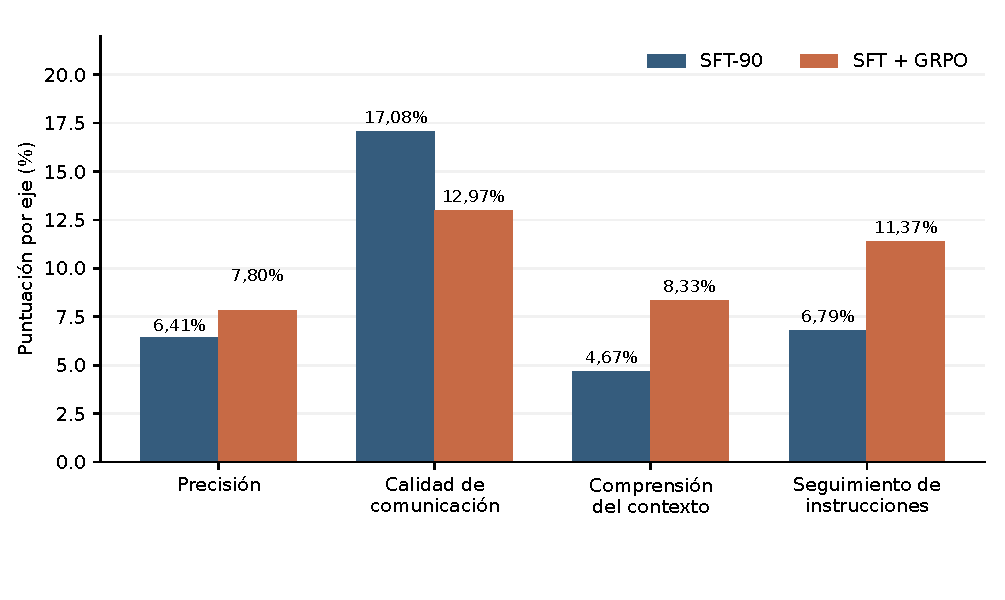
\includegraphics[width=\textwidth]{Figuras/04-resultados/resultados-ejes.pdf}
\caption{Comparación de SFT-90 y SFT-90 + GRPO en cuatro ejes.}
\label{fig:resultados-ejes}
\end{figure}

Como complemento, la tabla~\ref{tab:resultados-criterios} presenta los conteos no ponderados de los criterios positivos cumplidos y de los negativos activados. El modelo con GRPO cumplió 85 criterios positivos más, pero también activó 40 criterios negativos adicionales, de modo que el aumento de cobertura estuvo acompañado por una mayor frecuencia de comportamientos penalizados. Estos últimos incluyeron distintos tipos de errores y no se redujeron exclusivamente a problemas de seguridad clínica.

\begin{table}[htbp]
\centering
\caption{Cumplimiento de criterios sin ponderación por sus pesos.}
\label{tab:resultados-criterios}
\begin{tabularx}{\textwidth}{@{}Ccc@{}}
\toprule
Medida & SFT-90 & SFT-90 + GRPO \\
\midrule
Criterios positivos cumplidos & 626/4.003 & 711/4.003 \\
Proporción de positivos cumplidos & 15,64\% & 17,76\% \\
Criterios negativos activados & 672/1.736 & 712/1.736 \\
Proporción de negativos activados & 38,71\% & 41,01\% \\
\bottomrule
\end{tabularx}
\end{table}

La figura~\ref{fig:resultados-criterios} representa esas proporciones por separado, porque utilizaron denominadores distintos. Por tanto, no se sumaron como una puntuación única ni se equipararon con los resultados ponderados de los ejes, donde un criterio de mayor peso tuvo una contribución diferente de otro con menor peso.

\begin{figure}[htbp]
\centering
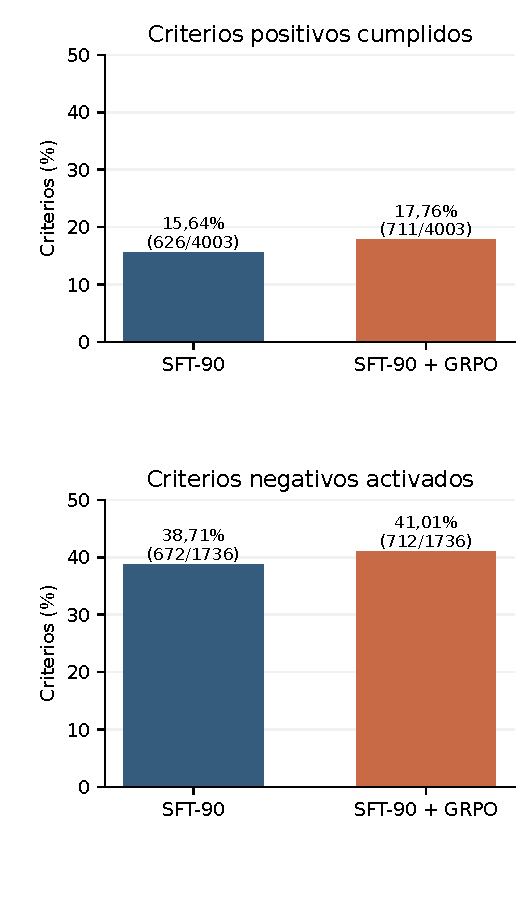
\includegraphics[width=8.9cm]{Figuras/04-resultados/resultados-criterios.pdf}
\caption{Criterios positivos cumplidos y negativos activados.}
\label{fig:resultados-criterios}
\end{figure}

\section{Contraste de la metodología con RaR}
\label{sec:comparacion-rar}
\label{sec:resultados-modelos}
La segunda etapa parte de Qwen2.5-3B SFT45k y estudia su adaptación con datos procedentes de RaR. Compararlo con Qwen2.5-7B SFT-90 o con su adaptación mediante GRPO no permitiría aislar el efecto de la metodología, porque también cambian la capacidad del modelo, la supervisión y los datos de aprendizaje. Por esa razón, los modelos de ambas etapas no son comparables entre sí.

La función de los experimentos iniciales es aportar evidencia sobre la metodología y orientar su refinamiento. Para estudiar los efectos de las nuevas rúbricas o de su puntuación, las comparaciones deberán realizarse dentro de la segunda etapa, manteniendo constantes las condiciones que no sean objeto del análisis. A su vez, el contraste con los resultados publicados de RaR estará condicionado por la equivalencia que pueda comprobarse en el protocolo, como se establece en la sección~\ref{sec:protocolo-segunda-etapa}.

El contraste con RaR se centra en la construcción de las rúbricas y en la forma de convertir sus evaluaciones en recompensa~\cite{gunjal2025rar}. Para interpretar las puntuaciones deben cotejarse el modelo, el SFT previo, los datos utilizados en RL y las condiciones del benchmark, la generación y el juez. Las diferencias que no puedan mantenerse constantes delimitan el alcance de esa comparación.

Los registros del piloto permiten analizar el entrenamiento descrito en la sección~\ref{sec:refinamiento-entrenamiento-rar}. La evaluación externa de esta etapa y su contraste numérico con los resultados publicados de RaR no se presentan todavía; por ello, las puntuaciones de HealthBench de la sección anterior corresponden únicamente a las pruebas iniciales con Qwen2.5-7B.

\section{Aciertos y errores en las respuestas generadas}
\label{sec:resultados-cualitativos}

El cuadro~\ref{tab:resultados-ejemplos} reúne cuatro ejemplos de diferencias favorables y desfavorables al modelo con GRPO, mediante fragmentos originales en inglés contrastados con las respuestas completas.

\begingroup
\renewcommand{\tablename}{Cuadro}
\singlespacing
\setlength{\parskip}{3pt}
\setlength{\tabcolsep}{4pt}
\begin{longtable}{|>{\centering\arraybackslash}p{0.27\textwidth}|>{\centering\arraybackslash}p{0.325\textwidth}|>{\centering\arraybackslash}p{0.325\textwidth}|}
\caption{Ejemplos de diferencias entre las respuestas evaluadas.}
\label{tab:resultados-ejemplos}\\
\hline
\textbf{Aspecto evaluado} & \textbf{SFT-90} & \textbf{SFT-90 + GRPO} \\
\hline
\endfirsthead
\hline
\textbf{Aspecto evaluado} & \textbf{SFT-90} & \textbf{SFT-90 + GRPO} \\
\hline
\endhead
\hline
\multicolumn{3}{|c|}{Continúa en la página siguiente.} \\
\hline
\endfoot
\hline
\endlastfoot
\textbf{Seguimiento de instrucciones}\par
Recomendaciones de dieta, ejercicio y consulta médica ante calambres.
&
\enquote{Take a good diet rich in calcium and magnesium.}
&
\enquote{Stretching exercises before and after physical activity can also help prevent muscle cramps.}
\\[0.3\baselineskip]
\hline
\textbf{Comprensión del contexto}\par
Indagación sobre la historia del problema de visión periférica borrosa.
&
\enquote{Please provide more details or rephrase your question.}
&
\enquote{Are you experiencing any other symptoms such as headaches, dizziness, or nausea?}
\\[0.3\baselineskip]
\hline
\textbf{Adecuación de la extensión}\par
Explicar brevemente el significado de contraindicación.
&
\enquote{Contraindication refers to a condition or factor that makes a particular treatment or procedure unsuitable or risky for a patient.}
&
\enquote{contraindications may include severe renal impairment, active infection, or other medical conditions}
\\[0.3\baselineskip]
\hline
\textbf{Criterio negativo}\par
Recomendaciones sin evidencia para prevenir el cólera.
&
\enquote{handwashing with soap, can help prevent the spread of the disease.}
&
\enquote{Adding a teaspoon of salt and a teaspoon of sugar for every 5 liters of water can help prevent diarrhea.}
\\
\end{longtable}
\endgroup

En la consulta sobre calambres, SFT incluyó dieta y consulta médica, y SFT + GRPO añadió ejercicios para cubrir las tres indicaciones. Ante la visión borrosa, formuló preguntas sobre síntomas asociados. Sin embargo, también agregó ejemplos innecesarios para definir contraindicación y una medida sin evidencia para el cólera, según el juez local.

Tras la adaptación supervisada, GRPO comparó varias respuestas por consulta y favoreció aquellas con mayor recompensa relativa, calculada mediante rúbricas que valoraron la recuperación de conceptos de referencia. La retirada gradual de ayudas buscó favorecer respuestas autónomas, un mecanismo compatible con la mayor cobertura observada, aunque su efecto causal no quedó demostrado.


\chapter{Contribuciones de la tesis}
\label{ch:contribuciones}

El trabajo reúne una propuesta metodológica, su implementación y una evaluación inicial en el dominio clínico. Los resultados disponibles corresponden a la primera etapa, mientras que la segunda desarrolla el refinamiento de las rúbricas y de la recompensa con datos procedentes de RaR. Por ello, las contribuciones distinguen la evidencia obtenida de los desarrollos posteriores y de los experimentos que todavía requieren ejecución y análisis.

\section{Integración metodológica}
\label{sec:contribuciones-integracion}
El trabajo implementa un procedimiento que utiliza respuestas de referencia para construir una señal de recompensa específica por consulta e incorporarla al entrenamiento con GRPO. En su aplicación inicial a HealthCareMagic e iCliniq, esa supervisión combina detección por código, revisión semántica y ayudas que se retiran durante el entrenamiento.

La evaluación en HealthBench permitió identificar diferencias entre recuperar más información y producir una respuesta mejor valorada en todas sus dimensiones. Este resultado orientó el refinamiento de los criterios: la segunda etapa parte de lo que solicita la pregunta y utiliza la referencia como evidencia para formular los requisitos, con una puntuación separada para criterios esenciales y adicionales.

El aporte metodológico reúne esa implementación y el refinamiento derivado de su evaluación. Los componentes, sus formulaciones y la configuración del entrenamiento se desarrollan en el capítulo~\ref{ch:metodo-propuesto}, mientras que el capítulo~\ref{ch:resultados-adaptacion} presenta los datos, el protocolo de evaluación y los resultados disponibles.


\section{Rúbricas específicas por consulta}
\label{sec:contribuciones-rubricas}
Las respuestas de referencia aportan contenido para construir criterios específicos por consulta y utilizarlos en el cálculo de recompensa. La primera etapa utiliza entidades y reglas compiladas, mientras que el piloto posterior incorpora obligaciones explícitas de la pregunta, criterios atómicos vinculados a evidencia, alternativas semánticas y revisión mediante IA. Estos desarrollos permiten documentar cómo se construye y se puntúa la supervisión, pero sus efectos sobre las respuestas del modelo requieren la evaluación prevista para la segunda etapa. En ambas etapas debe distinguirse la fidelidad a la referencia de una validación profesional de su corrección clínica.


\section{Evidencia sobre los alcances y límites}
\label{sec:contribuciones-evidencia}

Se evaluó Qwen2.5-7B SFT-90 frente a su adaptación posterior con GRPO sobre los mismos 500 casos de HealthBench. El modelo con GRPO cumplió más criterios positivos, pero también activó más criterios negativos y obtuvo una menor puntuación en calidad de comunicación. Estos resultados muestran que aumentar la cobertura de información puede introducir otros errores, por lo que la recompensa necesita considerar ambos efectos. La interpretación sigue limitada por las diferencias entre los jueces utilizados y los posibles sesgos de la evaluación local.

La combinación de mayor cobertura y más penalizaciones motivó revisar qué requisitos se incluyen en las rúbricas y cómo se ponderan en la recompensa de la segunda etapa.


\section{Implementación y trazabilidad}
\label{sec:contribuciones-implementacion}

La implementación separó el entrenamiento del servicio de evaluación y conservó las configuraciones, los registros de métricas y los checkpoints. Esto permitió revisar las decisiones del evaluador y relacionar los resultados con el modelo utilizado.

\section{Trabajo futuro y evaluación pendiente}
\label{sec:trabajo-futuro}
La continuación del trabajo se concentra en evaluar la segunda etapa bajo condiciones documentadas. Los registros de SFT45k y del piloto permiten analizar el aprendizaje descrito en el capítulo~\ref{ch:evolucion-entrenamiento}, mientras que la evaluación externa de la segunda etapa y el contraste con RaR requieren completarse. Por ello, las rúbricas preparadas y las configuraciones implementadas deben distinguirse de los resultados que todavía no se presentan.

En primer lugar, corresponde comprobar cómo los criterios construidos a partir de las obligaciones de la consulta se comportan ante respuestas correctas, parciales, contradictorias y equivalentes en significado. Esta revisión debe permitir calibrar al juez y detectar recompensas que favorezcan menciones superficiales o exigencias no solicitadas antes de interpretar una mayor puntuación como una mejora de las respuestas.

A continuación, las variantes de recompensa y de ayudas deberán compararse dentro de la segunda etapa, manteniendo constantes el modelo de partida, los datos y la evaluación. Estas comparaciones permitirán estudiar por separado el efecto de las rúbricas, de su puntuación y de las ayudas. El contraste con RaR también requiere comprobar las condiciones descritas en la sección~\ref{sec:comparacion-rar} y explicitar aquellas que no sean equivalentes.

Por último, el experimento final previsto en la sección~\ref{sec:protocolo-final-previsto} contempla un reparto del conjunto de aprendizaje en mitades para SFT y GRPO, con validación y prueba reservadas. Esta propuesta permitirá evaluar el procedimiento bajo una separación definida desde el inicio, pero no se considera ejecutada ni se confunde con el SFT45k o con el piloto preparado. Las curvas de entrenamiento y los resultados externos deberán incorporarse cuando estén disponibles y verificados.


\cleardoublepage
\chapter*{Bibliografía}
\addcontentsline{toc}{chapter}{Bibliografía}
\printbibliography[heading=none]
\end{document}
